%% 
%% Copyright 2007-2025 Elsevier Ltd
%% 
%% This file is part of the 'Elsarticle Bundle'.
%% ---------------------------------------------
%% 
%% It may be distributed under the conditions of the LaTeX Project Public
%% License, either version 1.3 of this license or (at your option) any
%% later version.  The latest version of this license is in
%%    http://www.latex-project.org/lppl.txt
%% and version 1.3 or later is part of all distributions of LaTeX
%% version 1999/12/01 or later.
%% 
%% The list of all files belonging to the 'Elsarticle Bundle' is
%% given in the file `manifest.txt'.
%% 
%% Template article for Elsevier's document class `elsarticle'
%% with numbered style bibliographic references
%% SP 2008/03/01
%% $Id: elsarticle-template-num.tex 272 2025-01-09 17:36:26Z rishi $
%%
\documentclass[preprint,12pt]{elsarticle}

%% Use the option review to obtain double line spacing
%% \documentclass[authoryear,preprint,review,12pt]{elsarticle}

%% Use the options 1p,twocolumn; 3p; 3p,twocolumn; 5p; or 5p,twocolumn
%% for a journal layout:
%% \documentclass[final,1p,times]{elsarticle}
%% \documentclass[final,1p,times,twocolumn]{elsarticle}
%% \documentclass[final,3p,times]{elsarticle}
%% \documentclass[final,3p,times,twocolumn]{elsarticle}
%% \documentclass[final,5p,times]{elsarticle}
%% \documentclass[final,5p,times,twocolumn]{elsarticle}

%% For including figures, graphicx.sty has been loaded in
%% elsarticle.cls. If you prefer to use the old commands
%% please give \usepackage{epsfig}

%% The amssymb package provides various useful mathematical symbols
\usepackage{amssymb}
%% The amsmath package provides various useful equation environments.
\usepackage{amsmath}
%% The amsthm package provides extended theorem environments
%% \usepackage{amsthm}
\usepackage{array}
\usepackage{tabularx}
\usepackage{booktabs}
\usepackage{algorithm}
\usepackage{algorithmic}
%% The lineno packages adds line numbers. Start line numbering with
%% \begin{linenumbers}, end it with \end{linenumbers}. Or switch it on
%% for the whole article with \linenumbers.
%% \usepackage{lineno}

\journal{Journal of Theoretical Biology}

\begin{document}

\begin{frontmatter}

%% Title, authors and addresses

%% use the tnoteref command within \title for footnotes;
%% use the tnotetext command for theassociated footnote;
%% use the fnref command within \author or \affiliation for footnotes;
%% use the fntext command for theassociated footnote;
%% use the corref command within \author for corresponding author footnotes;
%% use the cortext command for theassociated footnote;
%% use the ead command for the email address,
%% and the form \ead[url] for the home page:
%% \title{Title\tnoteref{label1}}
%% \tnotetext[label1]{}
%% \author{Name\corref{cor1}\fnref{label2}}
%% \ead{email address}
%% \ead[url]{home page}
%% \fntext[label2]{}
%% \cortext[cor1]{}
%% \affiliation{organization={},
%%             addressline={},
%%             city={},
%%             postcode={},
%%             state={},
%%             country={}}
%% \fntext[label3]{}

\title{Stability-Driven Assembly Theory}

%% use optional labels to link authors explicitly to addresses:
%% \author[label1,label2]{}
%% \affiliation[label1]{organization={},
%%             addressline={},
%%             city={},
%%             postcode={},
%%             state={},
%%             country={}}
%%
%% \affiliation[label2]{organization={},
%%             addressline={},
%%             city={},
%%             postcode={},
%%             state={},
%%             country={}}

\author{Dan Adler} %% Author name

%% Author affiliation
\affiliation{email={dan@danadler.com}}

%% Abstract
\begin{abstract}
The emergence of complexity and information remains a fundamental question spanning physics, chemistry, biology, and computation. While traditional approaches often describe information as an emergent property, they rarely explain how it dynamically arises from purely abiotic processes. This paper introduces Stability-Driven Assembly (SDA) systems, a theoretical framework that models pattern evolution through probabilistic interactions governed by differential stability. Our computational experiments demonstrate that stability differences alone can generate selection pressure, driving systems toward lower-entropy states characterized by dominant stable patterns—without requiring explicit replication mechanisms. Through controlled intervention experiments, we establish a causal relationship between stability constraints and system evolution, showing how stability functions as a control parameter that shapes the evolutionary landscape. The SDA framework reveals the interplay between bottom-up assembly processes and top-down selective pressures, where emergent stable patterns recursively influence future interactions. Dynamic network visualization and token flow analysis further illuminate how stability-driven selection operates across scales, from local interactions to global pattern distributions. These findings provide a mechanistic explanation for how complexity and information can emerge in abiotic systems, with implications for understanding prebiotic chemical evolution, self-organizing systems, and the transition from non-living to living matter.
\end{abstract}


%%Graphical abstract
\begin{graphicalabstract}
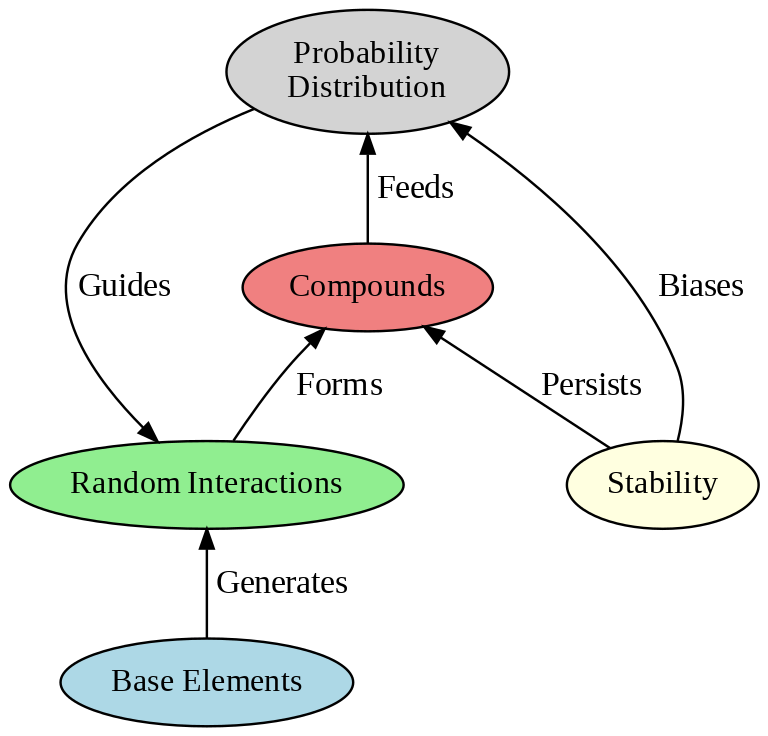
\includegraphics[width=1\textwidth]{figure_10}
\end{graphicalabstract}

%%Research highlights
\begin{highlights}
\item Establishes Stability-Driven Assembly (SDA) systems as a mathematical framework for modeling selection in abiotic systems.
\item Demonstrates through controlled intervention experiments the causal relationship between stability constraints and system evolution.
\item Proves that differential pattern persistence alone can generate evolutionary dynamics without explicit replication mechanisms.
\item Visualizes stability-driven selection through dynamic network representations and token flow analysis.
\item Provides a unifying framework for understanding pattern formation across chemical, physical, and information-processing systems.
\end{highlights}

%% Keywords
\begin{keyword}
Stability-driven selection; Abiotic evolution; Pattern formation; Emergent complexity; Entropy reduction; Evolutionary dynamics; Chemical evolution
\end{keyword}

 %% keywords here, in the form: keyword \sep keyword

%% PACS codes here, in the form: \PACS code \sep code

%% MSC codes here, in the form: \MSC code \sep code
%% or \MSC[2008] code \sep code (2000 is the default)

\end{frontmatter}

% The order of the section titles is different for some journals. Please refer to the "Instructions for Authors” on the journal homepage.

\section{Introduction}

"\textit{Selection for longevity becomes inseparable from selection for propagation. What persists has, by definition, a greater opportunity to propagate its structure.}" This observation by Stuart Kauffman \cite{kauffman1995home} identifies a fundamental principle that may bridge the gap between inanimate physical processes and biological evolution. The transition from non-living to living systems represents one of science's most profound questions, yet while the mechanisms of biological evolution through natural selection are well established, the emergence of selection itself—prior to true replication—remains enigmatic.

In inanimate physical systems, patterns persist according to their stability under prevailing conditions. A carbon lattice in diamond form persists longer than graphite under high pressure; certain molecular configurations outlast others in various chemical environments. This differential persistence creates an implicit selection mechanism—stable configurations naturally become more prevalent over time simply by outlasting less stable alternatives. This fundamental principle of stability-driven selection may have preceded and enabled the emergence of biological selection.

The study of such selection mechanisms spans multiple scientific disciplines. Algorithmic complexity \cite{kolmogorov1965complexity} and Shannon's information theory \cite{shannon1948mathematical} provide tools to quantify patterns and information, but do not explain how information emerges from physical systems. Constructor theory \cite{deutsch2013constructor} reframes physical laws in terms of possible transformations, while Assembly Theory (AT) \cite{walker2023nature} quantifies complexity through the minimal steps needed to construct an object, yet provides a retrospective rather than dynamic model of selection in real time.

Particularly relevant to stability-driven selection are autocatalytic sets, developed by Kauffman \cite{kauffman1986autocatalytic} and further explored by Hordijk and Filisetti \cite{hordijk2011required}, which examine how networks of molecules can collectively catalyze each other's production. Similarly, Fontana's Artificial Chemistry (AlChemy) \cite{fontana1991algorithmic} uses lambda calculus to model chemical reactions and explores how self-maintaining networks of interacting molecules emerge. The preferential attachment model introduced by Barabási and Albert \cite{barabasi1999emergence} demonstrates how entities with more connections preferentially attract new connections, creating a "rich-get-richer" effect conceptually similar to stability-driven selection, though based on connectivity rather than longevity.

This paper introduces Stability-Driven Assembly (SDA) systems as a theoretical framework to explore how selection based purely on differential stability can drive the emergence of complexity and information. By abstracting away specific physical laws, SDA systems model how persistent patterns accumulate, interact, and evolve through probabilistic processes guided by stability constraints. This approach offers a conceptual bridge between non-living physical systems governed by stability dynamics and the information-rich, evolutionary processes characteristic of biological systems.

Stability-Driven Assembly (SDA) systems distinguish themselves by their narrow focus on stability as the central determinant of pattern persistence. Stability is simulated by associating different lifetimes with concatenated patterns, capturing the essential dynamics of selection without invoking detailed physical or chemical laws. This approach allows SDA systems to isolate and model selection as the driving mechanism of pattern evolution. By emphasizing stability-driven selection in evolving state spaces, SDA systems provide a dynamic and generative framework for studying how patterns are created, maintained, and ultimately evolve into complex configurations, complementing existing approaches while filling a crucial gap in our understanding of how complexity emerges from simple principles.

While SDA systems share some characteristics with natural processes where differential persistence creates selection pressure, such as crystal formation, sand dune patterns, and river network evolution, they abstract away specific physical mechanisms to focus on the universal principle of stability-driven selection. This abstraction allows us to formulate testable predictions about pattern formation in prebiotic and chemical systems, including the emergence of pseudo-homochirality and plateau-like complexity transitions that could be detected in laboratory experiments.

\section{SDA System Fundamentals}

\subsection{System Description}

We define a Stability-Driven Assembly (SDA) system as a population of base elements \( A, B, C, \dots \) capable of forming compounds through local interactions. Compounds are represented as strings formed by concatenating base elements and existing compounds, allowing repetitive and recursive patterns of unbounded length. The elements may exist in our physical universe or in an abstract universe. 

The stability of compounds determines how many generations they will persist in the population. For example, if compound AAB has a stability of 10, it will persist for 10 generations before disappearing. Unlike bidirectional models like MAK where dissipation of patterns is modeled explicitly, SDA systems simply eliminate expired patterns. Since interactions are unconstrained, compounds with a stability of 0 may be created and destroyed in the same generation, effectively simulating impossible interactions. 

Base elements regenerate at a constant rate in each generation, ensuring a continuous influx of resources that prevents stagnation and enables sustained exploration of the state space. This mirrors the continuous-flow stirred tank reactor (CFSTR) methodology used in chemical reaction modeling, where reactants are replenished at a constant rate to maintain steady-state conditions \cite{fogler1999chemical}. For \( n \) base elements replenished at a rate of \( m \) copies per generation, \( n \cdot m \) new tokens are injected per generation, supplementing existing compounds which may interact multiple times per generation. The term "token" is used in analogy to Petri nets \cite{petri1962communication}, where tokens represent discrete entities that move through a network based on transition rules. In SDA systems, tokens track the presence of patterns evolving under stability-driven selection.

\begin{figure}[htp]
    \centering
    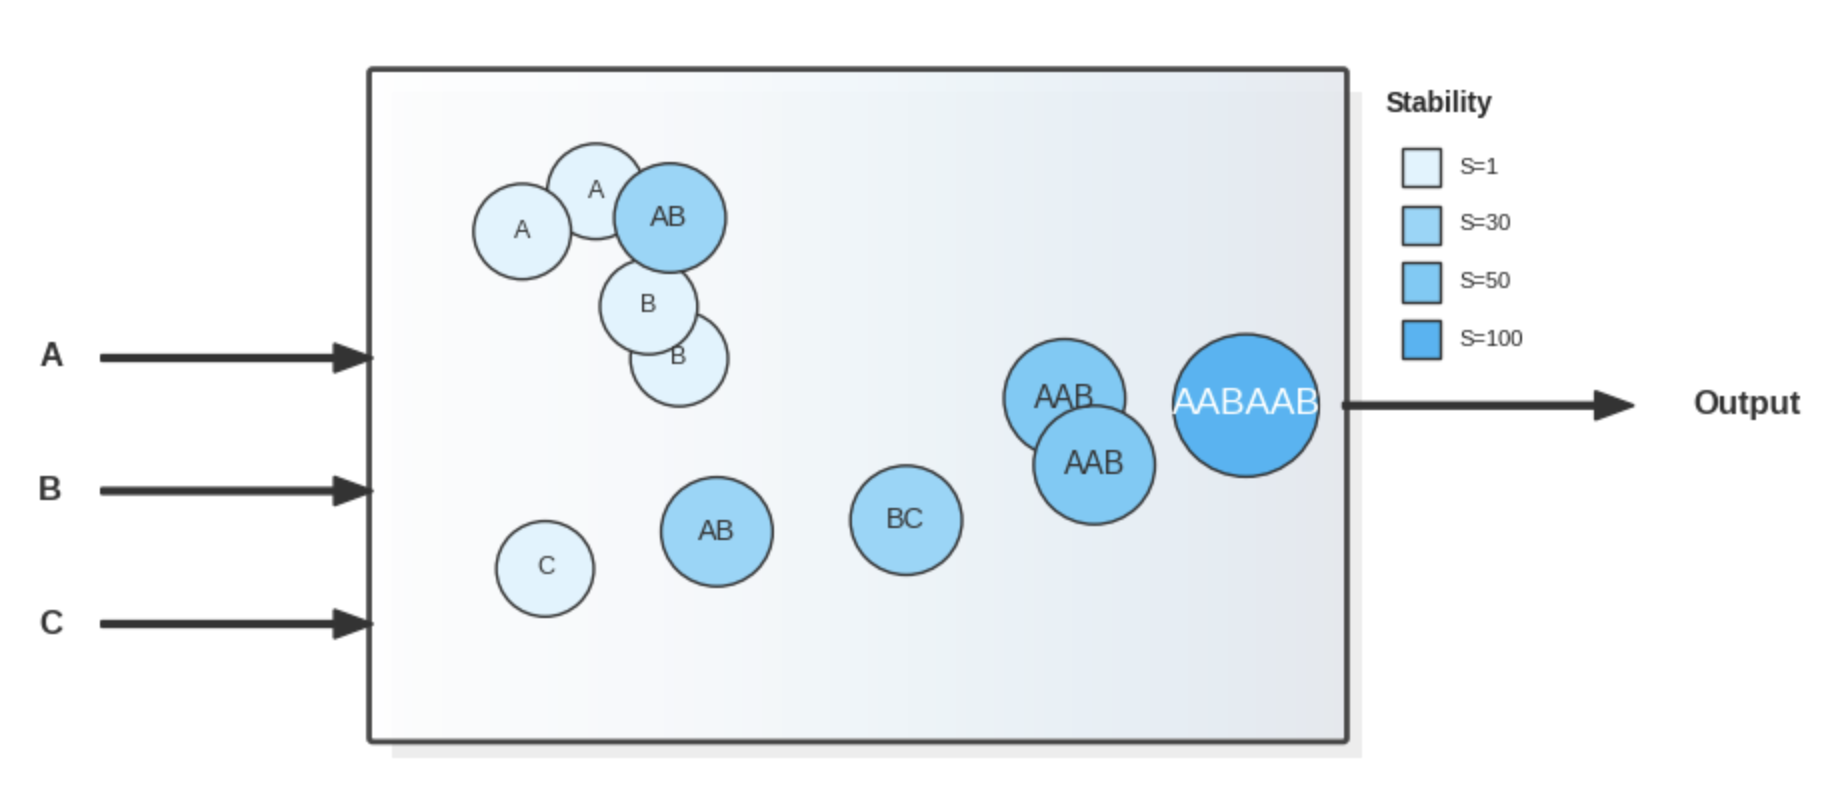
\includegraphics[height=5cm]{figure_1}
    \caption{SDA analogue of a chemical Continuous Flow Stirred Tank Reactor (CFSTR)}
    \label{fig:figure_1}
\end{figure}

\subsection{Formal Definition}

A Stability-Driven Assembly (SDA) system is formally defined as a tuple $(E, P, S, R, I)$ where:
\begin{itemize}
   \item $E = \{e_1, e_2, \ldots, e_n\}$ is a finite set of base elements
   \item $P$ is the set of all possible patterns formed by concatenating elements from $E$ and existing patterns, with each pattern $p \in P$ being a string over the alphabet $E$
   \item $S: P \rightarrow \mathbb{Z}^{+}$ is a stability function mapping each pattern to a non-negative integer representing its lifetime in generations
   \item $R: E \rightarrow \mathbb{Z}^{+}$ is a replenishment function specifying how many copies of each base element are added per generation
   \item $I \in \mathbb{Z}^{+}$ is the number of interactions allowed per generation
\end{itemize}

The state of the system at generation $t$ is defined by the set of patterns present in the population, with each pattern's presence implicitly determining its probability of selection for interactions. The pattern interaction operation, denoted by $\oplus$, is defined as string concatenation. When patterns $p_1$ and $p_2$ interact, they form pattern $p_1 \oplus p_2$.


\begin{algorithm}[H]
\caption{SDA System Simulation}
\begin{algorithmic}[1]
\REQUIRE Set of base elements $E$, stability function $S$, replenishment rates $R$, interaction count $I$, generations $T$
\ENSURE Evolution of pattern population over $T$ generations
\STATE Initialize population with base elements according to initial conditions
\FOR{$t = 1$ to $T$}
   \STATE Remove patterns that have reached their stability-determined expiration time
   \FOR{each element $e \in E$}
       \STATE Add $R(e)$ copies of element $e$ to the population
   \ENDFOR
   \FOR{interaction count from $1$ to $I$}
       \STATE Randomly select two patterns from the current population
       \STATE Form new pattern $p_{new}$ by concatenating the selected patterns
       \STATE Determine stability lifetime $S(p_{new})$ for the new pattern
       \STATE Add the new pattern to the population with creation time $t$ and expiration time $t + S(p_{new})$
   \ENDFOR
   \STATE Record population state for analysis (optional)
\ENDFOR
\RETURN Pattern population evolution
\end{algorithmic}
\end{algorithm}


The probability of selecting a pattern $p$ for interaction in generation $t$ is naturally proportional to its frequency in the population. This creates a statistical feedback mechanism: patterns with higher stability persist longer, becoming more abundant in the population, which increases their probability of participating in interactions and forming new compounds.

\subsection{Illustrative Examples}

Consider a simple SDA system starting with a few instances of the base elements \( A \) and \( B \). The pattern \( AB \) has a lifetime of 10 generations, while \( ABAB \) has a lifetime of 50 generations, and all other compounds degrade instantly with a lifetime of 0. After the first generation, the system produces combinations such as \( AA \), \( BB \), and \( AB \). Since \( AA \) and \( BB \) are unstable, they are eliminated, leaving \( A \), \( B \), and \( AB \). In subsequent generations, new unstable patterns may appear transiently, but \( AB \) persists due to its longer lifetime. The abundance of \( AB \) naturally increases as it persists, raising the probability of forming \( ABAB \). This dynamic reflects a form of roulette wheel selection \cite{goldberg1989genetic} \cite{holland1975adaptation}, where stability-driven persistence affects interaction probability. The emergent pattern \( ABAB \) represents a higher-order configuration, demonstrating how selection, grounded in differential stability, shapes the system's evolutionary pathways. 

The following simulation shows a different SDA system, with a population of 3 elements: {A, B, C}. Assume that the B compounds are more stable than those without B. Thus, patterns like BB, AB, BC, and ABC have a higher stability than AC, A, or C. Therefore, B compounds will persist for multiple generations, while all others will dissipate. The more stable B-compounds will interact more frequently as a result of their relative frequency, even though there is no replication or inheritance at the individual compound level. A snapshot of the simulation is shown in Figure \ref{fig:figure_2}.

\begin{figure}[htp]
    \centering
    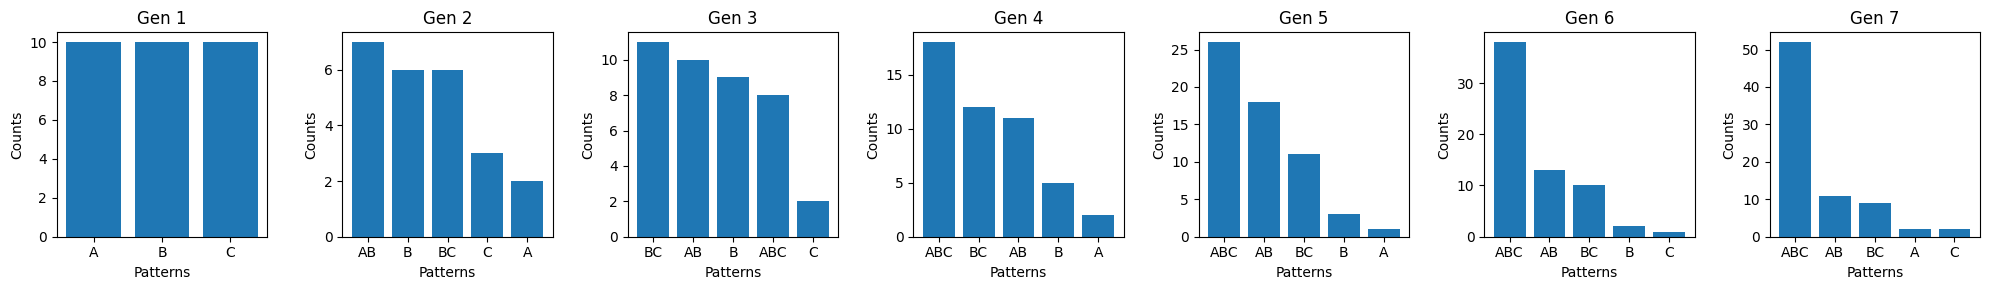
\includegraphics[width=1\textwidth]{figure_2}
    \caption{SDA System population evolution simulation}
    \label{fig:figure_2}
\end{figure}

Where is Maxwell's demon \cite{leff2002maxwell} hiding in Figure \ref{fig:figure_2}, driving it towards a low-entropy state? As we saw, the answer lies in the roulette wheel. Compounds that persist longer have more chances to interact. As their frequency in the population increases, their chances to interact grow even more. In Evolutionary Dynamics, this is called fitness-proportionate selection \cite{back1996evolutionary} or roulette wheel selection \cite{goldberg1989genetic} \cite{holland1975adaptation}.


\section{Analysis of SDA Systems Using Probability Distributions}

This section analyzes the behavior of SDA systems through probability theory, providing a mathematical framework for understanding how stability-driven selection shapes population dynamics over time.

\subsection{Population and Stability Distributions}

We can analyze SDA systems through two key distributions: the \textbf{population distribution}, which represents the relative abundance of patterns in the system, and the \textbf{stability distribution}, which quantifies pattern lifetimes. The population distribution at generation \( t \) can be defined as \( P_t(p) = \frac{N_t(p)}{\sum_{q \in P} N_t(q)} \), where \( N_t(p) \) is the count of pattern \( p \) at generation \( t \). This distribution evolves over time as patterns with different stabilities interact and persist.

The stability function \( S: P \rightarrow \mathbb{Z}^{+} \) maps each pattern to its lifetime in generations. Unlike the population distribution, which evolves dynamically based on interactions, the stability function is typically defined externally and remains constant throughout the simulation.

In applications to real-world scenarios, the values of \(S(p)\) would be determined by underlying physical, chemical, or other domain-specific principles. For example, in a chemical context, stability values might correspond to binding energies or activation barriers; in an economic model, they could represent market resilience or competitive advantage. The stability function encodes the persistence property that drives selection in SDA systems.

\subsection{Analytical Model of Pattern Dynamics}

To understand SDA system evolution analytically, we can model how pattern probabilities change across generations. The probability of observing pattern \(p\) at generation \(t+1\) results from two distinct processes: the persistence of existing copies and the creation of new copies through interactions.

For persistence analysis, we need to account for how pattern instances with different creation times contribute to the population. Given that pattern \(p\) has a deterministic lifetime of \(S(p)\) generations, we can express the persistence component as:

\begin{equation}
\label{eq:persist-term}
\mathrm{Persist}_t(p) = P_t(p) \cdot \left(1 - \frac{1}{\overline{R}_t(p)}\right)
\end{equation}

Where \(\overline{R}_t(p)\) represents the average remaining lifetime of pattern \(p\) instances in the population at generation \(t\), with \(\overline{R}_t(p) \leq S(p)\). This term accounts for the age distribution of existing pattern instances without assuming uniform creation rates.

When the system is far from equilibrium or experiencing rapidly changing dynamics, \(\overline{R}_t(p)\) may vary significantly between generations. In a perfectly stable system with a constant creation rate, \(\overline{R}_t(p)\) would approach \(\frac{S(p)+1}{2}\), the average of remaining lifetimes for uniformly distributed ages.

For creation analysis, we can estimate the probability of forming new copies of pattern \(p\) through concatenations:
\begin{equation}
\label{eq:create-term}
\mathrm{Create}_t(p) = \sum_{(q,r) \to p} P_t(q) \cdot P_t(r)
\end{equation}

Where the notation \((q,r) \to p\) indicates pattern pairs that, when concatenated, form pattern \(p\). For example, pattern ABA can form from AB+A or A+BA.

Combining these processes and normalizing yields an analytical approximation of the expected population distribution at the next generation:
\begin{equation}
\label{eq:full-ba-update}
P_{t+1}(p) = \frac{
  \mathrm{Persist}_t(p) + \mathrm{Create}_t(p)
}{
  \sum_{p' \in P} 
  \left[
    \mathrm{Persist}_t(p') + \mathrm{Create}_t(p')
  \right]
}
\end{equation}

It is important to note that this analytical model approximates the behavior of the SDA simulation rather than defining it. The actual simulation proceeds according to the algorithm defined earlier, while this model helps us understand and predict the statistical properties of the system.

\subsection{Entropy Dynamics Analysis}
Analysis of Equation~\ref{eq:full-ba-update} reveals two competing processes determining probability shifts across generations:
\begin{equation}
P_{t+1}(p) \propto \mathrm{Persist}_t(p) + \mathrm{Create}_t(p)
\end{equation}

An alternative approach to understanding entropy dynamics in SDA systems involves analyzing the rate of change in Shannon entropy over time. We can express the expected entropy change between generations as:
\begin{equation}
\Delta H = H(P_{t+1}) - H(P_t)
\end{equation}

For systems with varying pattern stabilities, the entropy dynamics are governed by the relative influence of persistence versus creation mechanisms. We can formalize this through an influence parameter $\alpha$, which represents the proportion of pattern abundance determined by stability-driven persistence:
\begin{equation}
\alpha = \frac{\sum_p \mathrm{Persist}_t(p)}{\sum_p \mathrm{Persist}_t(p) + \sum_p \mathrm{Create}_t(p)}
\end{equation}

When $\alpha$ approaches 1, stability-driven selection dominates the system dynamics; when $\alpha$ approaches 0, random creation processes predominate.

The entropy change can then be approximated as:
\begin{equation}
\Delta H \approx (1 - \alpha) \cdot \Delta H_{create} + \alpha \cdot \Delta H_{persist}
\end{equation}

Where $\Delta H_{create}$ represents the entropy change from creation processes (typically positive or zero) and $\Delta H_{persist}$ represents the entropy change from stability-driven persistence (typically negative).

\subsubsection{Simulation Results}
To empirically validate the entropy dynamics in SDA systems, we conducted a series of simulations comparing SDA systems to unconstrained systems. Figure~\ref{fig:entropy_comparison} shows the entropy evolution in both systems over time.

\begin{figure}[h]
    \centering
    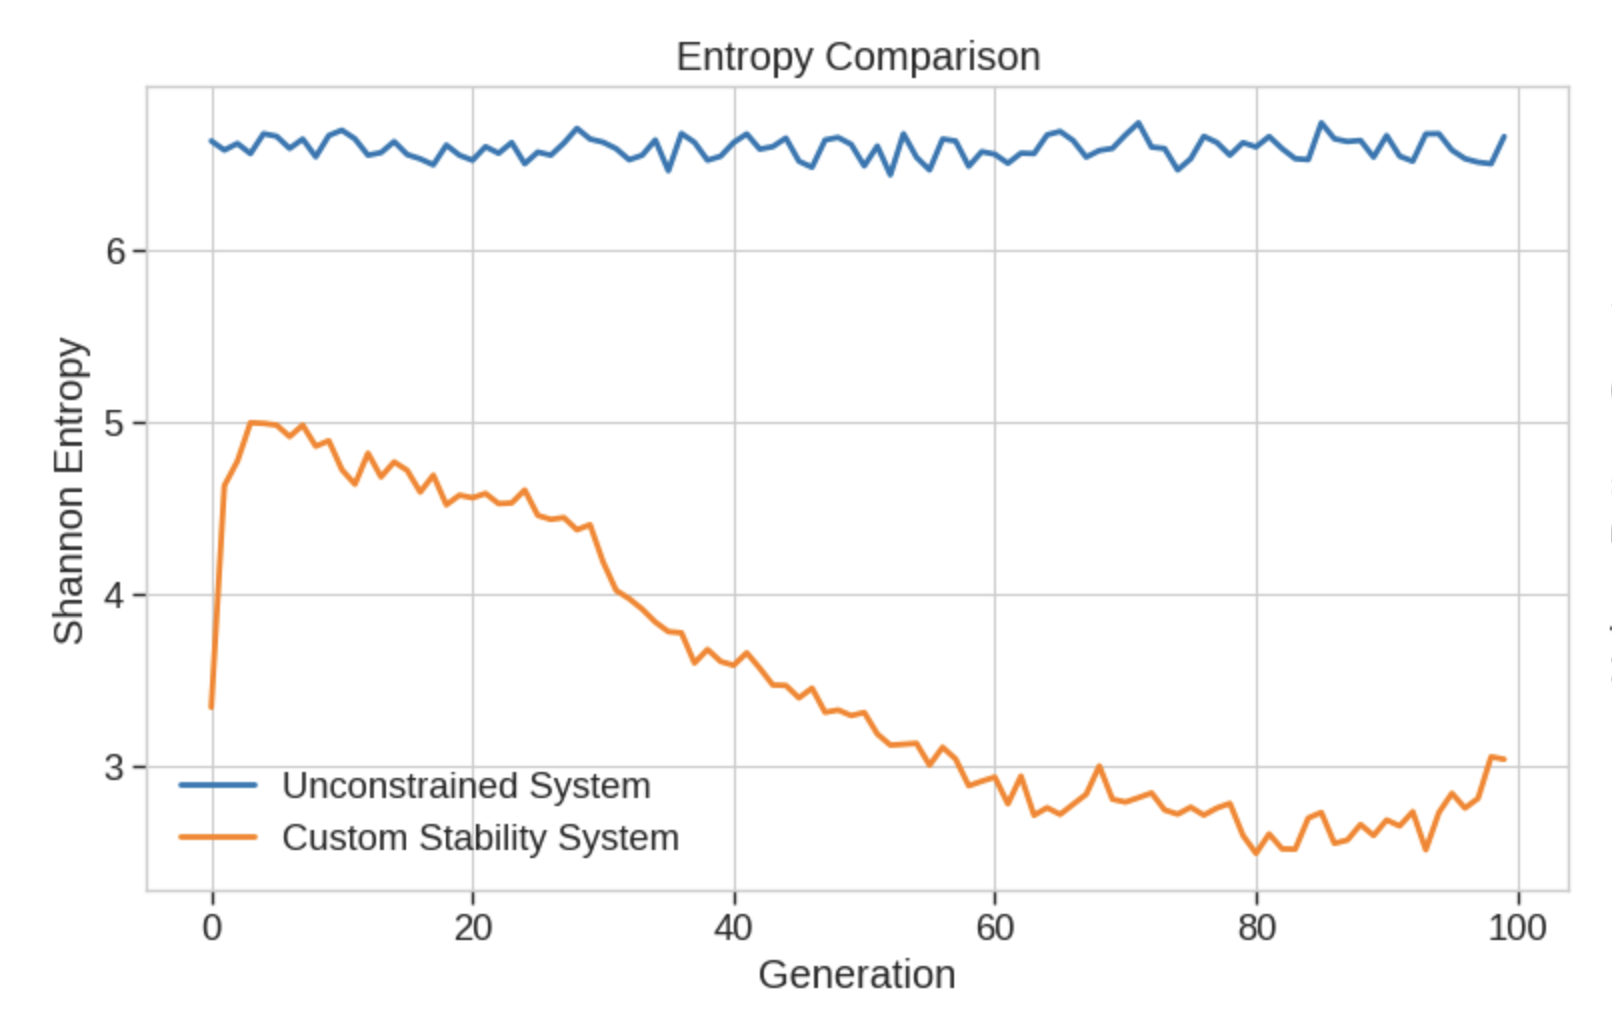
\includegraphics[width=0.8\textwidth]{entropy_comparison}
    \caption{Entropy comparison between SDA system and unconstrained system. The SDA system consistently maintains lower entropy due to stability-driven selection.}
    \label{fig:entropy_comparison}
\end{figure}

As predicted by our theoretical model, the SDA system demonstrates significantly lower entropy compared to the unconstrained system. The pattern diversity is also reduced, with high-stability patterns dominating the population. Figure~\ref{fig:pattern_distribution} illustrates this difference in pattern distributions.

\begin{figure}[h]
    \centering
    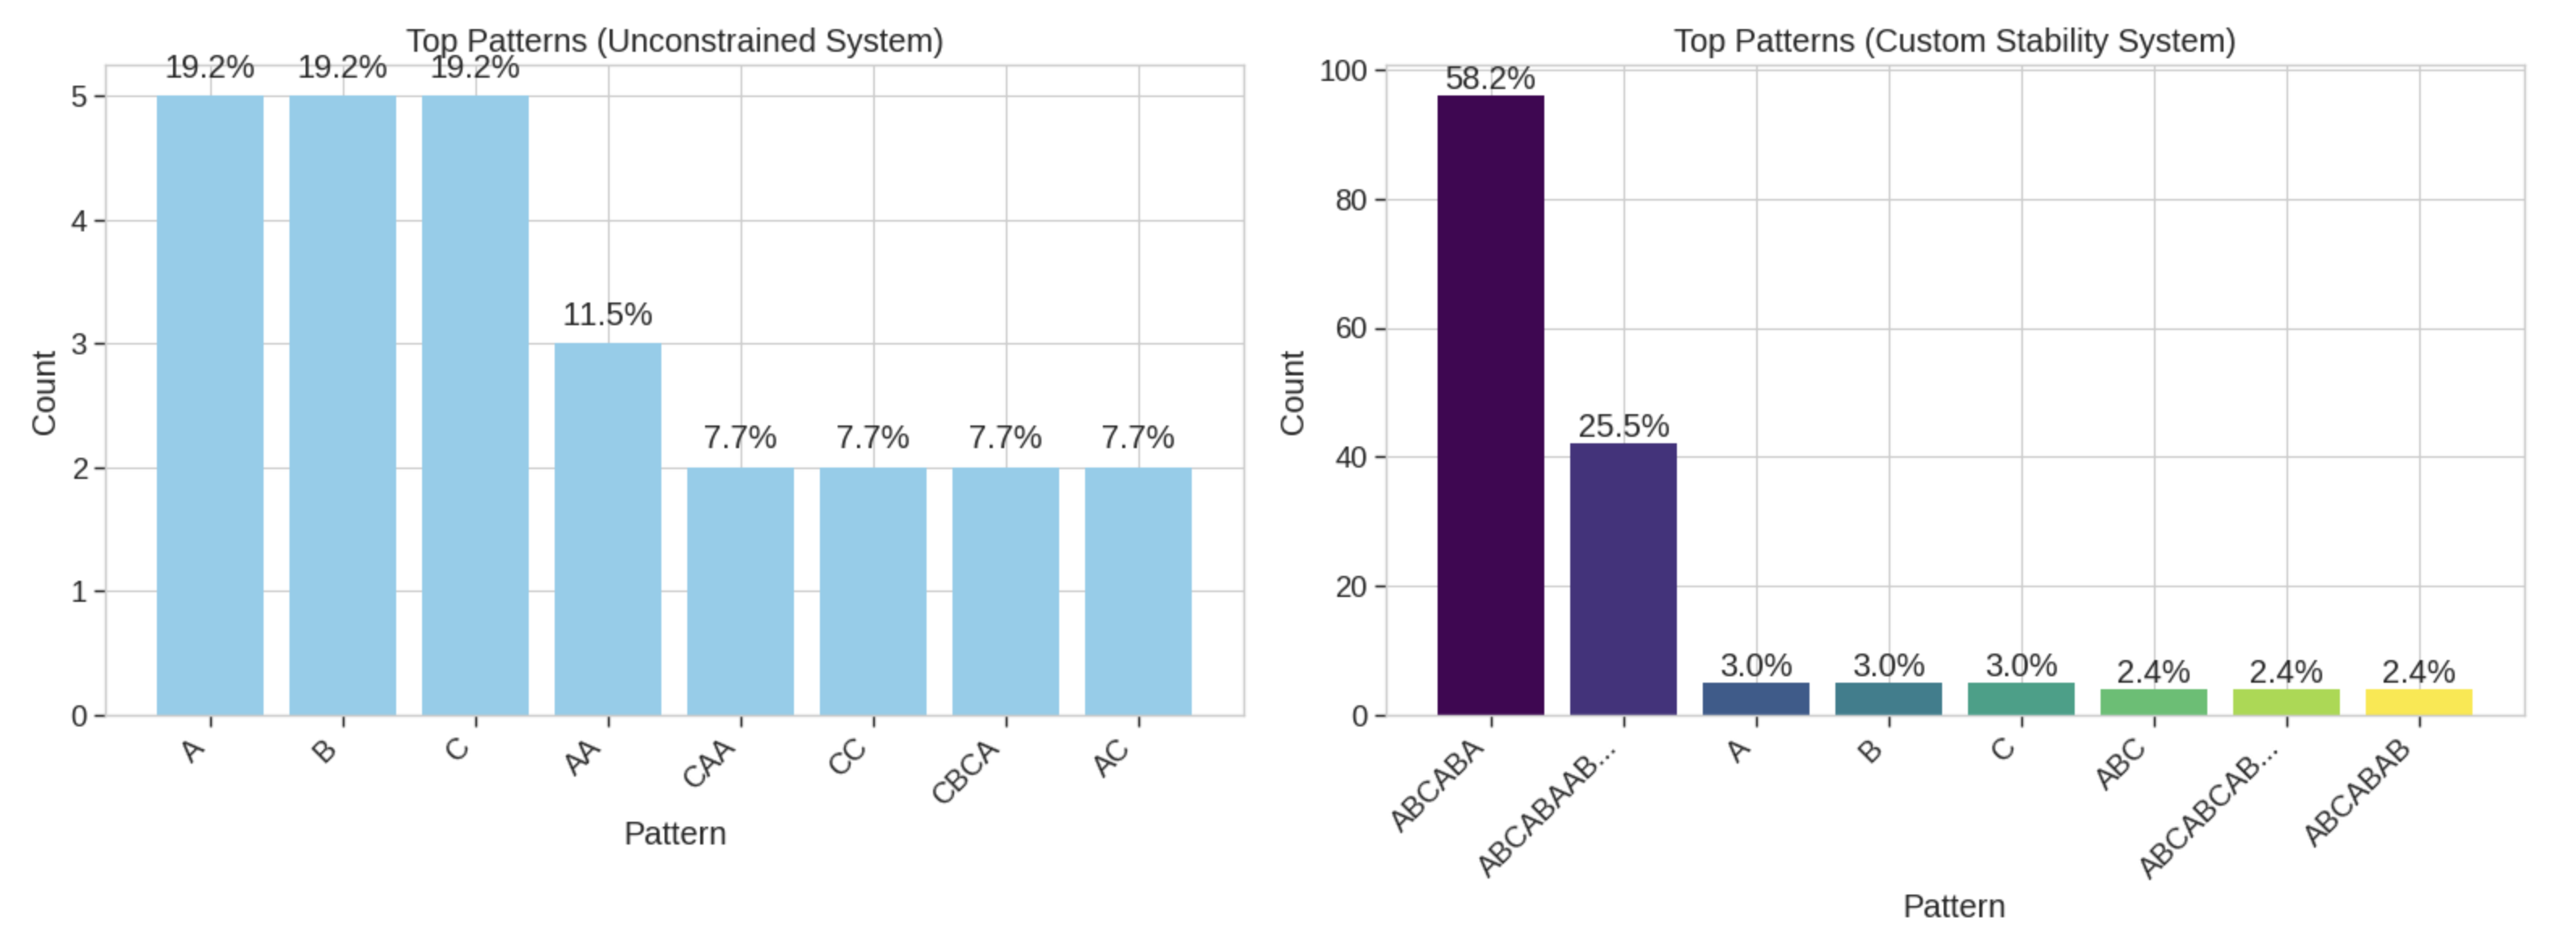
\includegraphics[width=1\textwidth]{pattern_distribution}
    \caption{Pattern distribution comparison. The SDA system (right) shows dominance of a few stable patterns, while the unconstrained system (left) exhibits a more uniform distribution, with base element replenishment rate of 5 dominating.}
    \label{fig:pattern_distribution}
\end{figure}

Interestingly, our simulations revealed that SDA systems with multiple high-stability patterns often exhibit oscillatory behavior in entropy over time. Figure~\ref{fig:entropy_oscillations} demonstrates this phenomenon.

\begin{figure}[h]
    \centering
    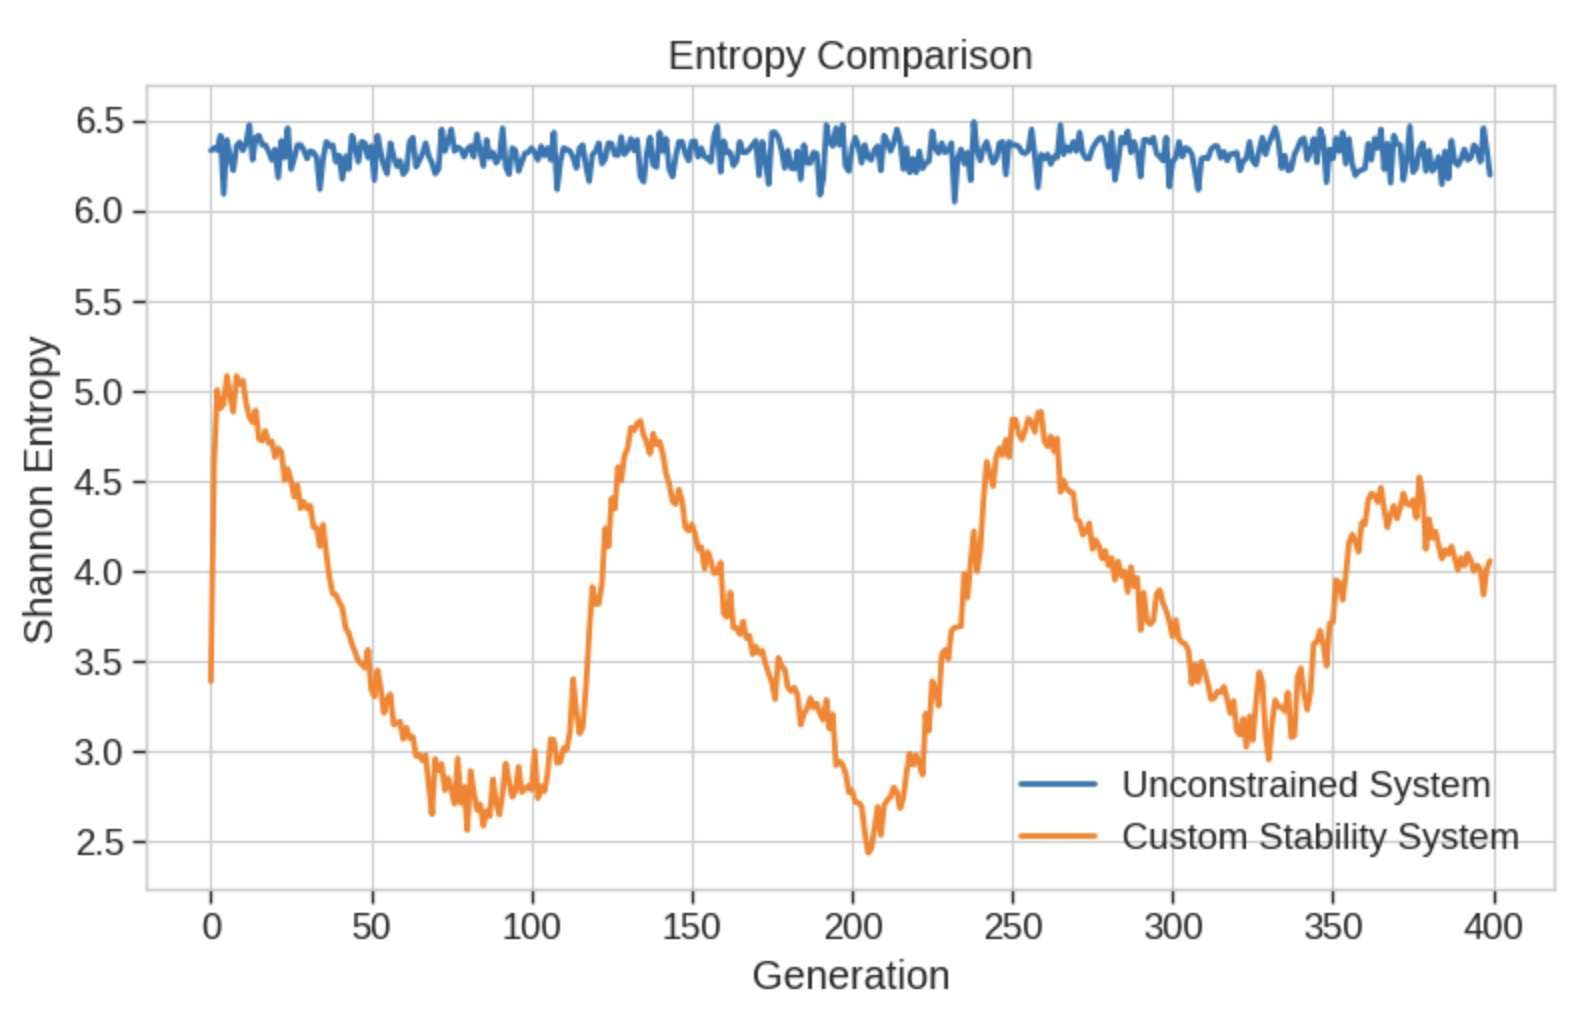
\includegraphics[width=0.8\textwidth]{entropy_oscillations}
    \caption{Oscillatory entropy dynamics in an SDA system with multiple high-stability patterns. The periods between entropy minima (marked with triangles) correspond to cycles of pattern dominance shifts.}
    \label{fig:entropy_oscillations}
\end{figure}

\subsubsection{Dynamical Systems Interpretation}
The oscillatory behavior observed in SDA systems bears striking resemblance to coupled oscillator networks analyzed by Strogatz \cite{strogatz2001exploring}. Drawing from complex network theory, we can interpret SDA systems as networks where patterns are nodes with intrinsic frequencies determined by their stability values.

In such systems, Strogatz demonstrates that oscillations emerge with periods that scale according to the relationship:

\begin{equation}
T \propto \sqrt{\frac{K}{|\omega_1 - \omega_2|}}
\end{equation}

Where $K$ is the coupling strength and $\omega_1$ and $\omega_2$ are the natural frequencies of interacting components. Adapting this framework to SDA systems, we propose that oscillation periods can be approximated by:

\begin{equation}
T \approx \beta \sqrt{\frac{I \cdot S_1 \cdot S_2}{|S_1 - S_2|}}
\end{equation}

Where $I$ is the interaction rate per generation, $S_1$ and $S_2$ are the stabilities of the dominant patterns, and $\beta$ is a system-specific constant. This formulation provides a theoretical basis for understanding the oscillatory dynamics observed in our simulations and connects SDA systems to the broader field of complex network theory.

The presence of these oscillations further demonstrates that SDA systems exhibit rich, complex dynamics driven by the interplay between pattern formation and stability-driven selection. These dynamics allow the system to explore different regions of the pattern space while maintaining lower entropy than unconstrained systems.

\section{Intervention Analysis of Stability-Driven Assembly Systems}

To test the causal relationship between stability constraints and system evolution, we conducted controlled intervention experiments on SDA systems. These experiments systematically altered stability parameters mid-simulation, allowing us to isolate the direct impact of stability on pattern distribution, entropy, and complexity. By comparing transitions from unconstrained to stability-driven configurations and vice versa, we established a rigorous basis for understanding how stability shapes evolutionary dynamics in these systems.

\subsection{Experimental Design}

We implemented two key intervention experiments:

\begin{enumerate}
    \item \textbf{Unconstrained to SDA}: An initially unconstrained system (uniform stability values) was allowed to evolve for 400 generations, after which stability constraints were introduced according to a predefined stability function $S(p)$ that assigned higher values to specific patterns.
    
    \item \textbf{SDA to Unconstrained}: An initially stability-constrained system evolved for 400 generations before having all stability constraints removed, setting all patterns to uniform stability values.
\end{enumerate}

In both cases, we maintained identical parameters for base element replenishment (rate = 5) and interaction frequency (100 interactions per generation). The stability function for the SDA condition assigned significantly higher values to certain patterns:

\begin{equation}
S(p) = 
\begin{cases}
100, & \text{if } p = \text{ABCABA} \\
50, & \text{if } p \in = \text{ABA, ABC} \\
30, & \text{if } p \in \{\text{AB, BC}\} \\
1, & \text{otherwise}
\end{cases}
\end{equation}

This differential stability created strong selection pressure favoring patterns with higher persistence values. Population metrics were tracked throughout the experiments, with special attention to system entropy, pattern diversity, and the relative abundance of specific pattern types before and after intervention.

\subsection{Unconstrained to SDA Transition}
\label{subsec:unconstrained-to-sda}

When transitioning from an unconstrained to a stability-driven regime, we observed pronounced and immediate changes in system behavior. Figure~\ref{fig:u2s-entropy} illustrates the entropy evolution across this transition point.

\begin{figure}[h]
    \centering
    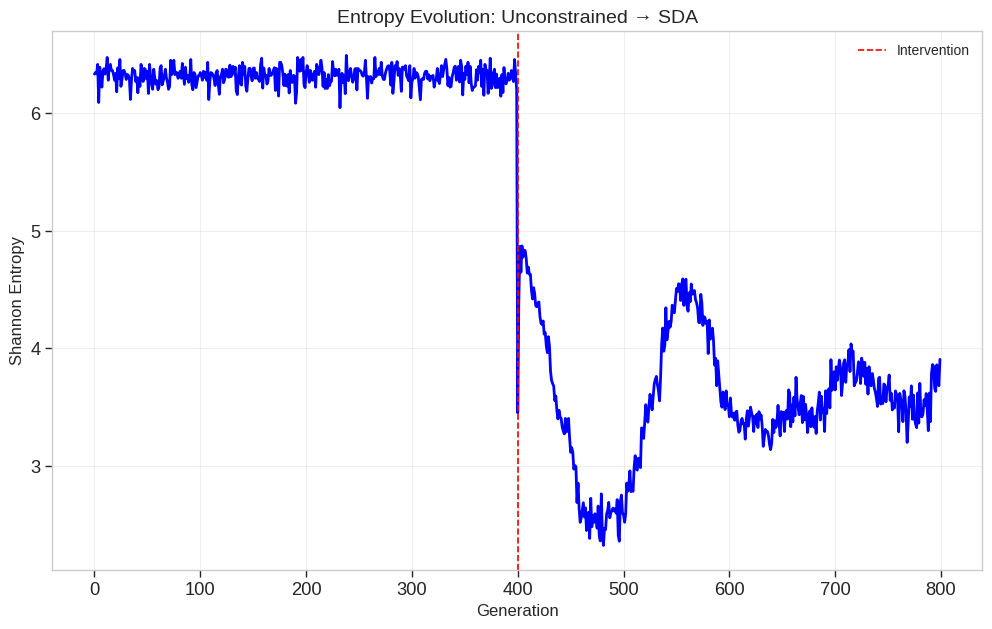
\includegraphics[width=1\textwidth]{unconstrained_to_sda_entropy.png}
    \caption{Entropy evolution when transitioning from an unconstrained to an SDA system. The vertical dashed line marks the intervention point where stability constraints were introduced.}
    \label{fig:u2s-entropy}
\end{figure}

\begin{figure}[h]
    \centering
    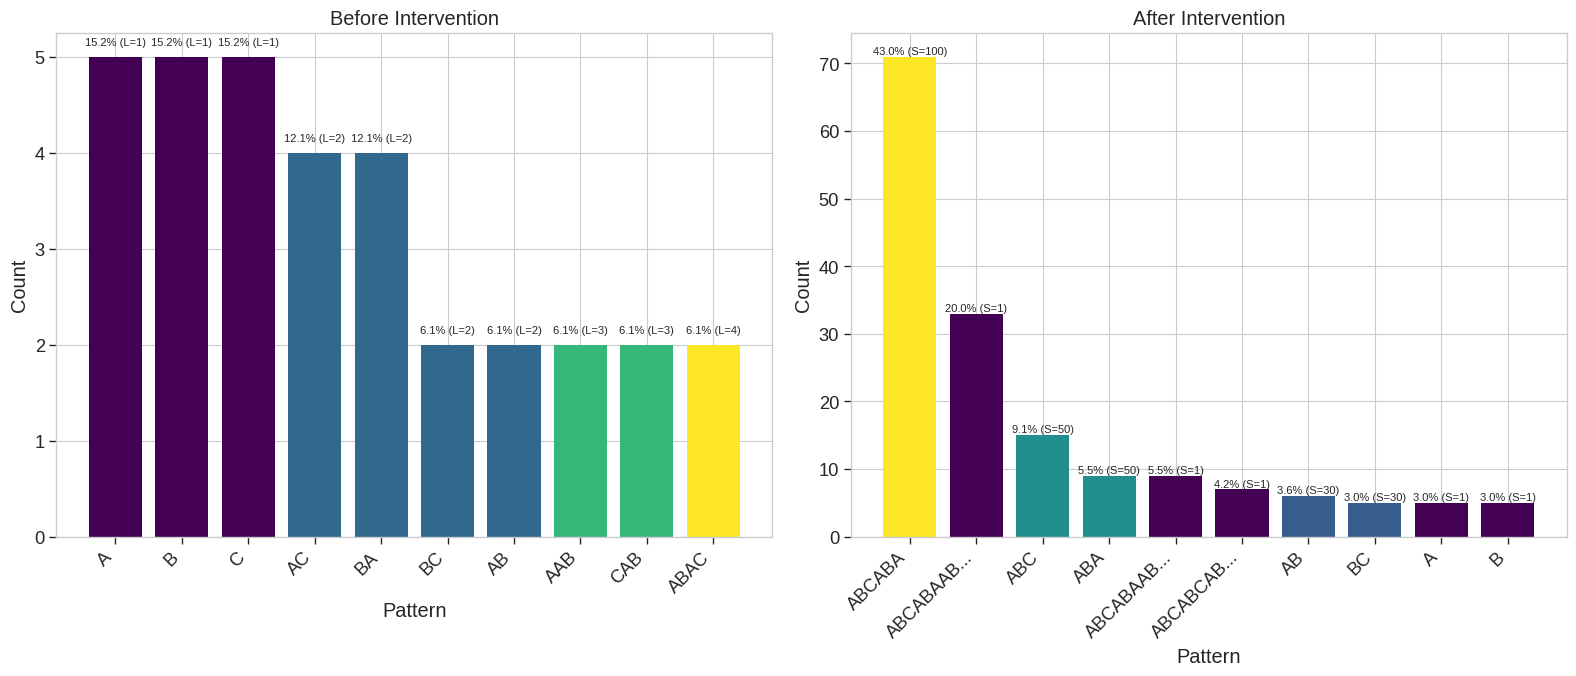
\includegraphics[width=1\textwidth]{unconstrained_to_sda_population_comparison.png}
    \caption{Pattern composition before (left) and after (right) transitioning from an unconstrained to an SDA system. Bar colors represent stability values, with darker colors indicating higher stability. Percentages indicate relative population frequency.}
    \label{fig:u2s-patterns}
\end{figure}


Prior to intervention, the system exhibited high entropy characteristic of an unconstrained regime, where all patterns persist for identical durations regardless of composition. After imposing the stability function at generation 400, entropy decreased rapidly and significantly before settling into some oscillations as described earlier. The pattern composition before and after intervention (Figure~\ref{fig:u2s-patterns}) reveals the mechanism behind this entropy change.

In the unconstrained phase, pattern distribution remained relatively uniform with numerous patterns maintaining similar population percentages. After introducing stability constraints, the system evolved toward dominance by patterns with higher assigned stability values. This supports the prediction in SDA theory that stability acts as a selective force.

\subsection{SDA to Unconstrained Transition}
\label{subsec:sda-to-unconstrained}

To establish bidirectional causality, we also examined the transition from a stability-driven to an unconstrained regime. Figure~\ref{fig:s2u-entropy} shows the entropy evolution during this reverse intervention.

\begin{figure}[h]
    \centering
    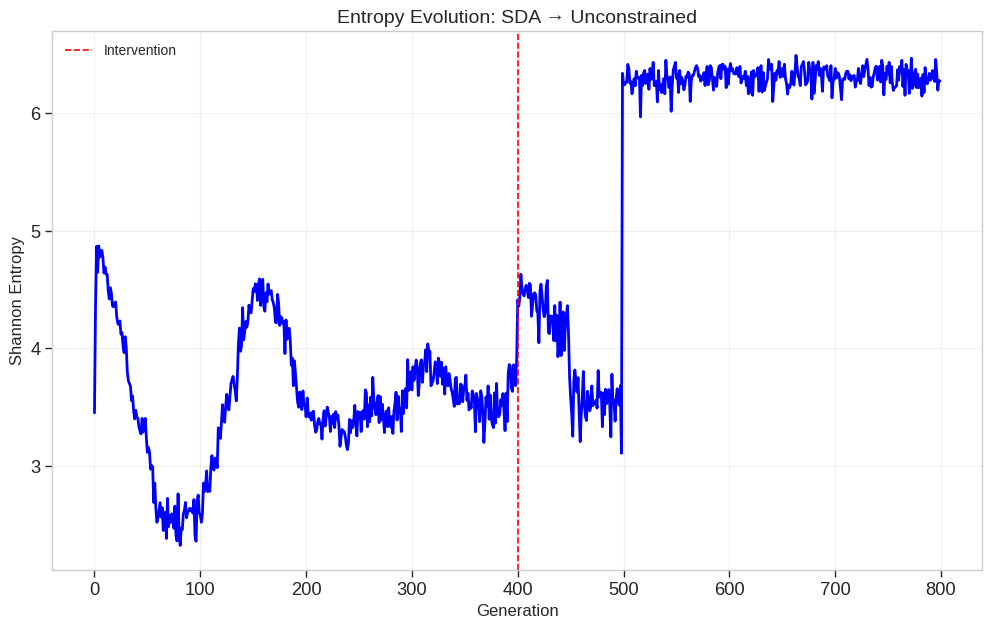
\includegraphics[width=1\textwidth]{sda_to_unconstrained_entropy.png}
    \caption{Entropy evolution when transitioning from an SDA to an unconstrained system. The vertical dashed line marks the intervention point where stability constraints were removed.}
    \label{fig:s2u-entropy}
\end{figure}

\begin{figure}[h]
    \centering
    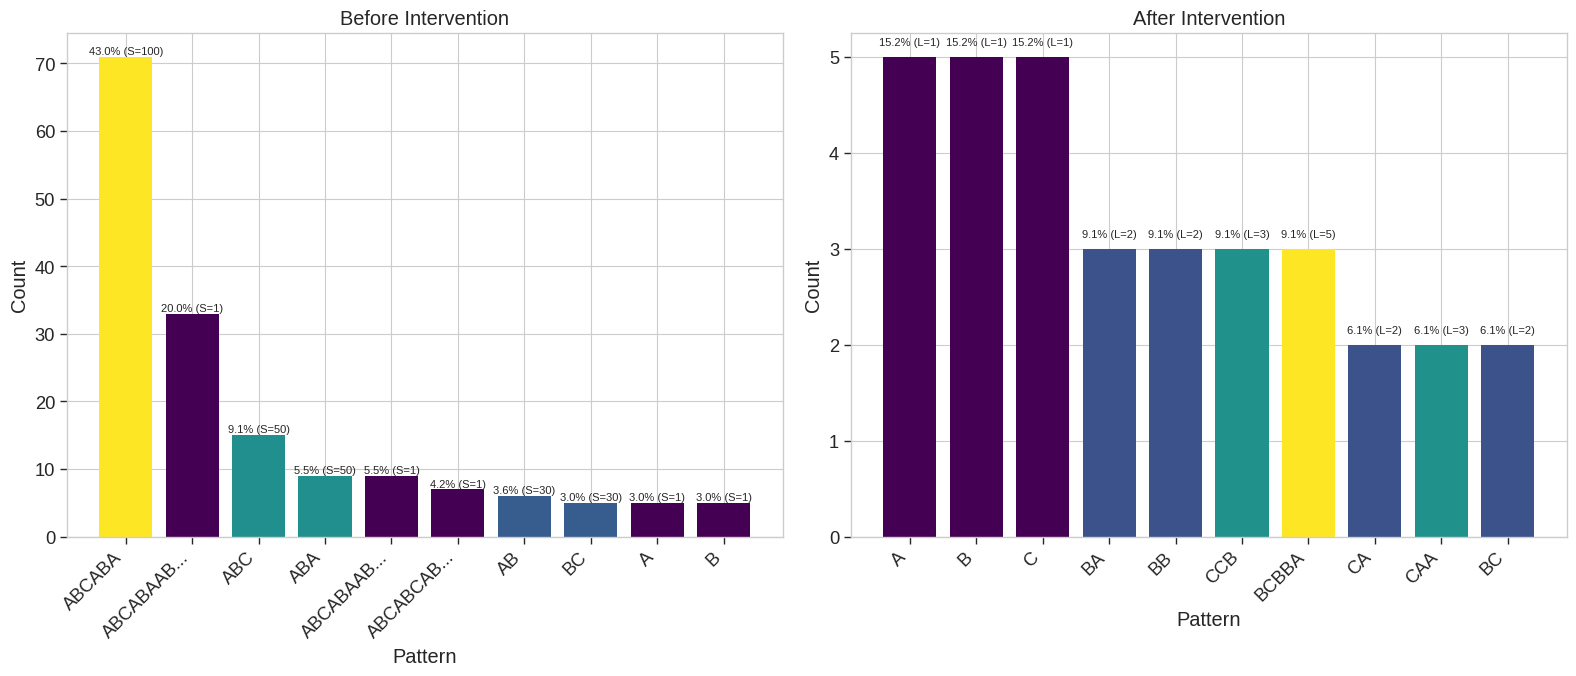
\includegraphics[width=1\textwidth]{sda_to_unconstrained_population_comparison.png}
    \caption{Pattern composition before (left) and after (right) transitioning from an SDA to an unconstrained system. Bar colors represent stability values in the SDA phase (left) and pattern length in the unconstrained phase (right).}
    \label{fig:s2u-patterns}
\end{figure}


Before intervention, the SDA system oscillated around low entropy values of ~4 bits, characterized by a distribution heavily skewed toward high-stability patterns. Upon removal of stability constraints at generation 400, entropy increased within 100 generations as stable patterns died out, and the system returned to a more uniform distribution with an entropy of over 6 bits. This confirms that entropy reduction in SDA systems is directly caused by differential stability rather than other factors. Figure~\ref{fig:s2u-patterns} displays the pattern composition before and after this reverse intervention.

The pre-intervention state shows the characteristic peaked distribution of the SDA system, with high-stability patterns dominating the population. After removing stability constraints, this distribution flattened considerably, as patterns previously favored solely for their stability lost their selective advantage. The pattern diversity increased from 47 unique patterns in the SDA regime to 129 in the unconstrained system, further demonstrating how stability constraints channel system evolution.

\subsection{Comparative Analysis and Causal Inference}
\label{subsec:comparative-analysis}

Figure~\ref{fig:combined-entropy} presents a comparative analysis of both intervention types, clearly establishing the causal relationship between stability constraints and entropy dynamics.

\begin{figure}[h]
    \centering
    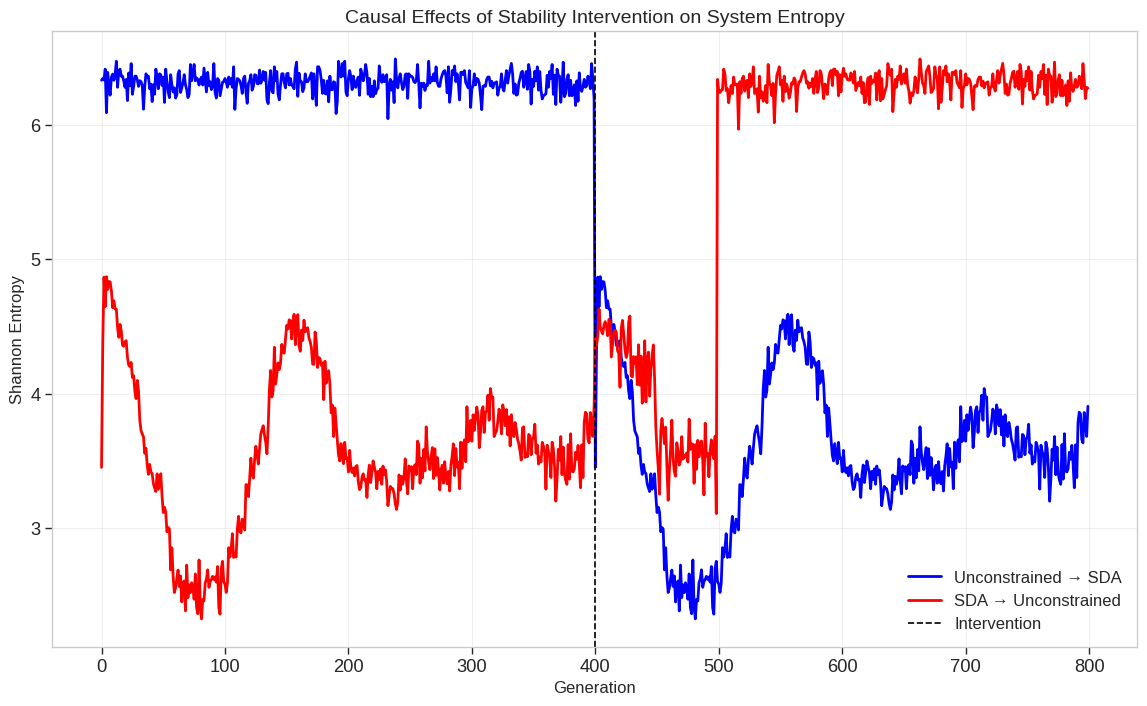
\includegraphics[width=0.9\textwidth]{combined_interventions.png}
    \caption{Comparative entropy evolution for both intervention types: unconstrained to SDA (blue) and SDA to unconstrained (red). The vertical line indicates the intervention point at generation 200.}
    \label{fig:combined-entropy}
\end{figure}

The symmetrical and opposite responses to intervention in both experiments provide strong evidence for causality. When stability constraints are imposed, entropy decreases; when they are removed, entropy increases. This symmetry suggests that stability acts as a control parameter that directly determines the entropy state of the system.

\subsection{Implications for Stability-Driven Assembly Theory}
\label{subsec:implications}

These intervention experiments provide several key insights into Stability-Driven Assembly Theory:

\begin{enumerate}
    \item \textbf{Causal Mechanism}: Stability differences directly cause the emergence of selection pressure, with no need for explicit replication mechanisms. The differential persistence of patterns based on their stability values is sufficient to generate evolutionary dynamics.
    
    \item \textbf{Entropy Reduction}: SDA systems naturally evolve toward lower-entropy states, with the magnitude of reduction proportional to the disparity in stability values between patterns.
    
    \item \textbf{Attractor States}: The system converges toward well-defined attractor states characterized by the dominance of high-stability patterns, demonstrating how stability acts as a control parameter that shapes the evolutionary landscape.
    
    \item \textbf{Reversibility}: The effects of stability-driven selection are reversible, confirming that the observed pattern distributions are maintained by ongoing selection pressure rather than historical contingency.
\end{enumerate}

These findings establish that stability-driven selection can account for the emergence of ordered, non-random pattern distributions without requiring explicit replication or inheritance mechanisms at the pattern level. By preferentially preserving certain configurations based solely on their persistence properties, SDA systems provide a minimal framework for understanding how complexity and information can accumulate in systems far from equilibrium.


\subsection{Evolutionary Dynamics in SDA Systems}
\label{subsec:evolutionary-dynamics}

A fundamental question arising from our intervention experiments is whether SDA systems genuinely evolve, or if "evolution" merely serves as an analogy. Evolution in biological systems typically involves replication, inheritance, and selection—processes that collectively produce adaptation over time. Although SDA systems lack explicit self-replication at the level of individual pattern instances, our intervention experiments reveal population-level dynamics that are mathematically indistinguishable from classical evolutionary processes.

The causal mechanism identified in Section~\ref{subsec:comparative-analysis} demonstrates how statistical feedback emerges naturally from differential stability. When the system transitions from unconstrained to stability-driven dynamics, patterns with higher stability consistently rise to dominance without requiring explicit replication machinery. As shown in Figure~\ref{fig:u2s-patterns}, high-stability patterns like ABCABA (stability = 100) increased from negligible representation to over 40\% of the population after stability constraints were introduced. This dominance emerges through two reinforcing mechanisms observed in our simulations:
\begin{enumerate}
    \item \textbf{Persistence advantage}: Higher stability patterns persist longer before being removed from the population, accumulating more copies over time.
    \item \textbf{Frequency-dependent selection}: As patterns become more frequent in the population, they have proportionally more opportunities to participate in interactions, further amplifying their representation.
\end{enumerate}

These dynamics align precisely with the principles of fitness-weighted selection in evolutionary systems, where persistence and reproductive opportunity drive the emergence of dominant patterns. The selection mechanism in SDA systems operates through what is effectively a roulette wheel selection process, where a pattern's probability of being selected for interaction is proportional to its frequency in the population, which in turn depends on its stability-determined lifetime.

The entropy changes observed after interventions in both directions (Figures~\ref{fig:u2s-entropy} and~\ref{fig:s2u-entropy}) confirm that this selection pressure continuously shapes the population distribution. When stability constraints were removed, previously dominant patterns quickly lost their selective advantage, demonstrating that their prevalence was maintained by ongoing selection rather than historical contingency.

Based on these empirical observations, we may assert that SDA systems exhibit genuine evolutionary behavior, not as a mere analogy, but as a mathematical inevitability arising from differential persistence. This conclusion is particularly significant because it suggests that selection—one of the core mechanisms of evolutionary change—can emerge spontaneously in systems with nothing more than (1) elements that can combine to form compounds, (2) differential stability among those compounds, and (3) probabilistic interaction rules.

The implications extend beyond theoretical interest: if selection can emerge spontaneously from stability differences, then evolutionary dynamics may be more universal than previously recognized, potentially operating in prebiotic chemical systems, planetary formation processes, and other non-biological contexts where structures with different lifetimes interact to form new compounds. The intervention experiments presented here provide empirical support for this broader view of evolutionary processes, establishing stability-driven selection as a potential bridge between non-living physical systems and the information-rich evolutionary processes characteristic of biological systems.


\section{Top-Down vs.\ Bottom-Up Dynamics in SDA Systems}
\label{sec:topdown-bottomup}

Figure~\ref{fig:figure_10} illustrates the interplay between top-down and bottom-up causation in Stability-Driven Assembly (SDA) systems, where the top-down influence emerges from the increasing relative abundance of stable patterns directing subsequent interactions, while bottom-up processes arise from the probabilistic assembly of base elements into intermediate and complex patterns, creating a dynamic feedback loop that drives the evolution of information and complexity.

\begin{figure}[h]
    \centering
    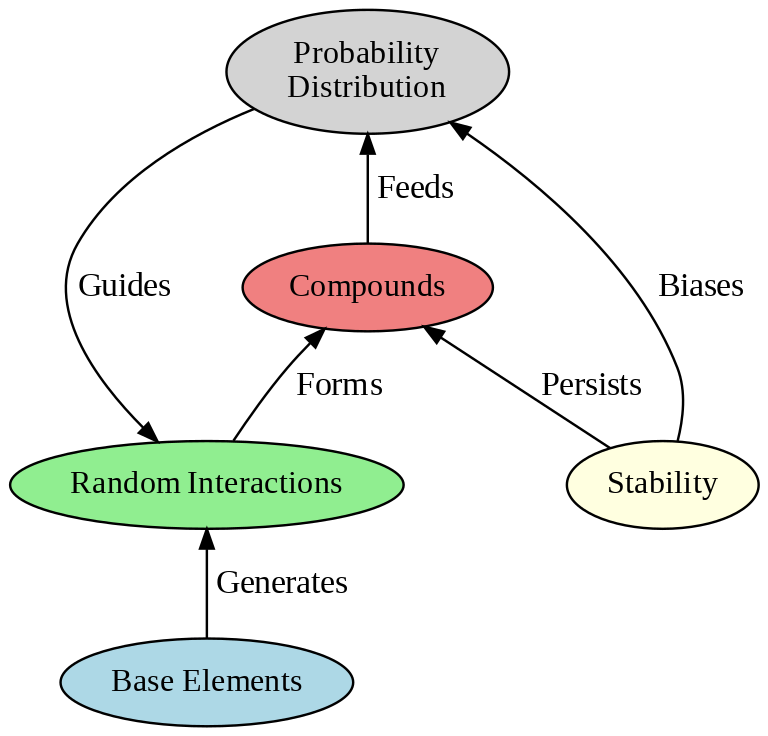
\includegraphics[width=0.7\linewidth,height=0.7\linewidth]{figure_10.png}
    \caption{Bottom-up and Top-down causation in SDA systems}
    \label{fig:figure_10}
\end{figure}

Once certain patterns become dominant, they exert a top-down influence on subsequent generations. These higher-level persistent structures shape future interactions by catalyzing or constraining the formation of new patterns. Hence, SDA systems do not just accumulate complexity through local rules; they also incorporate feedback from emergent structures that guide (or ``select for'') new configurations. The presence of memory and evolutionary history in these feedback loops distinguishes SDA systems from frameworks in which higher-level states simply describe aggregates without influencing the underlying microstates.

The contrast with traditional statistical mechanics is instructive \cite{landau1980statistical}. In statistical mechanics, macrostates (e.g., temperature, pressure) represent aggregate properties of microstates but do not directly influence the fundamental interaction rules among particles. In SDA systems, however, dominant patterns exert a causal influence on micro-level interactions, embedding history and specificity into the generative process itself. This dynamic distinguishes SDA systems by allowing feedback mechanisms that shape pattern evolution, separate from physical energy distributions or equilibrium constraints.

Such an explicit interplay between bottom-up and top-down dynamics in SDA systems suggests a broader principle for understanding complexity: emergent structures can become causal agents that direct further evolution of the system. This perspective helps explain the accumulation of novel order in contexts ranging from prebiotic chemistry to computational networks, where higher-level assemblies (compounds, motifs, or functional components) increasingly govern local interactions, thereby catalyzing the exploration of new possibilities for growth and adaptation.

At times, these dynamics appear teleological, as if the system were ``seeking'' more stable or more complex configurations. Bertalanffy \cite{bertalanffy1968general} cautions that such optimization processes, while suggestive of goal-directed behavior, often reflect nothing more than the natural unfolding of selection, feedback loops, and probability gradients rather than true purposeful design. SDA systems likewise illustrate how feedback from emergent structures can drive the exploration of new system states without implying an external or predetermined goal. By capturing both bottom-up and top-down mechanisms in an evolving distribution, SDA systems provide a model for understanding how complexity can accumulate, whether in prebiotic chemistry or in computational and informational domains, through iterative processes of selection and the continual reshaping of local interactions.

\section{Visualizing SDA Dynamics: Graph Representation and Application Examples}

Building on the intervention experiments that established the causal role of stability in pattern evolution, we now explore alternate representations and applications of SDA systems. While the numerical simulations quantify the emergence of selection pressure and entropy reduction, visualizing these dynamics through network representations offers additional insights into how stability shapes the flow of patterns through the system.


\subsection{Dynamic Graph Representation and Token Flow Analysis}

To further investigate the dynamics of SDA systems, we represent the state of the system in a specific generation as a directed graph, where the nodes correspond to base elements and compounds such as $A$, $AB$, $ABA$, $ABC$, and the directed edges represent the interactions that occurred between them in their assembly process. The base elements $A$, $B$, $C$ are replenished in each generation, initiating a cascade of interactions that propagate tokens (shown in Figure~\ref{fig:figure_5} as the count $N$ of instances or copies of each pattern). 

The token flow describes the redistribution of these tokens between nodes in the reaction graph, driven by stability dynamics and interactions. This process is analogous to probability currents in quantum mechanics \cite{feynman1965quantum} and optimal transport \cite{villani2008optimal}, reflecting the macroscopic evolution of the system. The tokens accumulate at nodes based on the flow dynamics, which are governed by the stability of each pattern (shown in Figure~\ref{fig:figure_5} as $S$), influencing the persistence and selection of patterns over successive generations.


\begin{figure}[h]
    \centering
    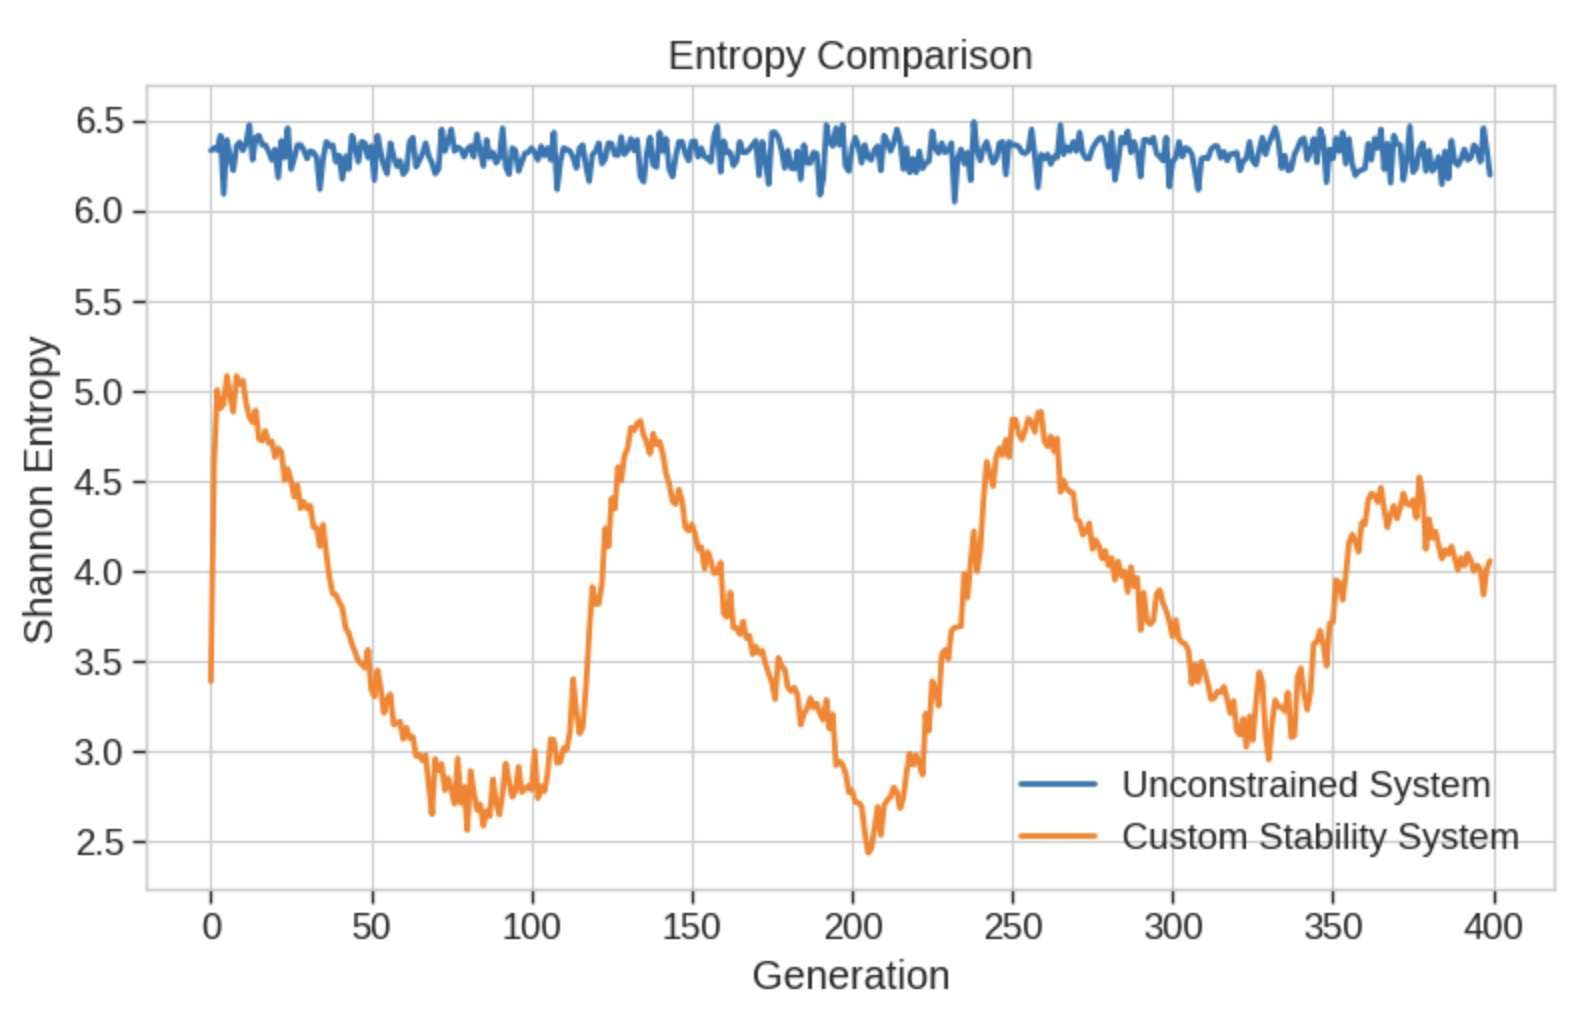
\includegraphics[width=0.7\linewidth]{figure_5.png}
    \caption{Graph representation of a SDA system showing stability (S), and the number of instances or tokens (N) of each base element and compound.}
    \label{fig:figure_5}
\end{figure}

The distribution of tokens across the graph reveals insights into the self-reinforcing nature of stability in SDA systems. Nodes with higher stability values (\textit{e.g.}, $ABCABA$) attract more tokens, leading to the emergence of dominant patterns. This phenomenon reflects a feedback loop: As tokens accumulate at a stable node, it becomes increasingly likely to dominate subsequent interactions, establishing preferential flow paths through the graph. Consequently, the system's token traffic converges to well-defined routes, concentrating resources on a subset of high-stability patterns while marginalizing less stable ones.

However, the graph may change significantly between generations if a new disruptor node emerges in the system. A disruptor node is characterized by a high stability value and strategic positioning within the graph, enabling it to compete with previously dominant nodes for token traffic. This disruptor can reroute flows, effectively redistributing tokens and breaking established dominance patterns. The behavior of token flows in the SDA system parallels physical phenomena, such as those observed in fluid systems, where a new high-conductivity channel can divert flow away from existing pathways. Similarly, in RC circuits, the introduction of a new low-resistance branch redistributes the current, altering the overall system equilibrium. 

Dynamic graphs have been used for switch-level simulation of transistor networks \cite{AdlerCAD}, where graph pathways are dynamically determined by the state of the on transistors, enabling specific connections to guide current flow. Similarly, in SDA systems, token flow is governed by stability and probabilistic interactions, determining which nodes persist and propagate.

\subsection{Application Examples of SDA Systems}

The SDA framework can be applied to model various real-world processes where stability-driven selection shapes the emergence of patterns. Below, we present two examples from different domains to illustrate the versatility of this approach.

\subsubsection{Chemical Example: Iron Oxidation}

\begin{figure}[h]
    \centering
    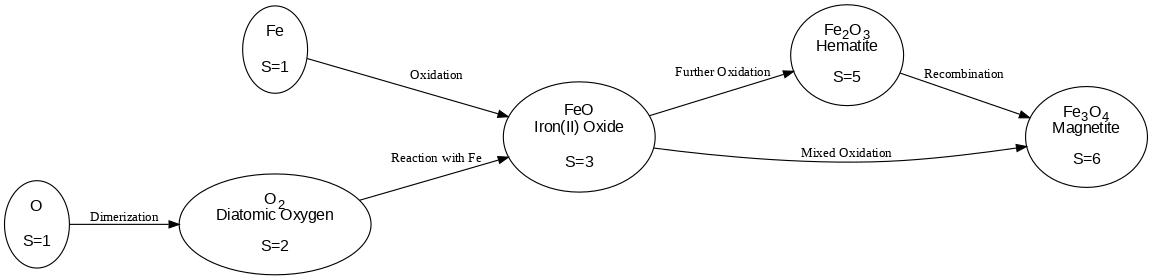
\includegraphics[width=1\textwidth,height=0.4\textwidth]{figure_6.png}
    \caption{Reaction network for iron oxidation, illustrating the stepwise formation of stable and intermediate compounds under stability constraints.}
    \label{fig:figure_6}
\end{figure}

The principles of Stability-Driven Assembly can be illustrated through the oxidation of iron, a realistic and naturally occurring chemical process. As shown in Figure~\ref{fig:figure_6}, iron oxidation (\(Fe\)) proceeds through a network of reactions driven by stability constraints. Oxygen (\(O\)) forms diatomic oxygen (\(O_2\)), which reacts with iron to produce a series of oxides, including iron(II) oxide (\(FeO\)), iron(III) oxide (\(Fe_2O_3\), hematite), and iron(II,III) oxide (\(Fe_3O_4\), magnetite). These reactions represent a progression from less stable intermediates to thermodynamically favored compounds. Competing pathways, such as partial oxidation or the formation of unstable intermediates, illustrate how stability shapes the evolution of the system, favoring reactions that lead to more persistent and energetically favorable products.

In the SDA framework, node stability \(S(p)\) quantifies the persistence of each compound, with higher stability values assigned to products such as hematite and magnetite due to their robust bonding and lower susceptibility to dissociation. This reaction network provides a testable system for validating the role of stability in driving reaction pathways. By simulating token flow dynamics based on stability values, the framework captures how high-stability compounds emerge and dominate over successive generations, aligning with experimental observations of oxidation processes.

\subsubsection{Economic Example: Industry Ecosystem as a SDA System}

\begin{figure}[h]
    \centering
    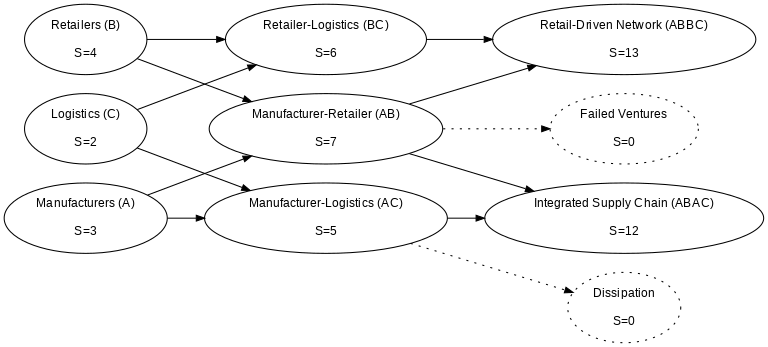
\includegraphics[width=1\textwidth]{figure_9.png}
    \caption{Industry ecosystem represented as a SDA system, showing the evolution from base businesses (\( A, B, C \)) to partnerships and stable integrated networks (\( ABAC, ABBC \)).}
    \label{fig:figure_9}
\end{figure}

This example illustrates a Stability-Driven Assembly system applied to an economic context, where the base elements represent different types of business. Manufacturers (A), retailers (B), and logistics providers (C) act as base elements with stabilities \( S_A, S_B, S_C \) reflecting their persistence in the market. Through successive interactions, these base elements form partnerships \( AB \), \( AC \), \( BC \) and evolve into integrated networks \( ABAC \), \( ABBC \), as shown in Figure~\ref{fig:figure_9}. Each stage corresponds to increasingly complex collaborations, where stability-driven selection ensures the persistence of dominant nodes. 

Stable nodes, such as \( AB \) (manufacturer-retailer) and \( ABBC \) (retail-driven networks), act as attractors, accumulating resources (tokens) over generations. Less stable nodes, including failed ventures (\( S=0 \)), dissipate quickly, redistributing tokens to more viable configurations. The economic analogy emphasizes how stability influences token flow, resource allocation, and the formation of hierarchical networks in complex systems. The tokens in this graph (individual companies) will naturally flow to configurations that are more stable and persistent, representing more business opportunities.

These examples from chemistry and economics demonstrate how the SDA framework provides a unifying perspective on pattern formation and selection across diverse domains. In each case, stability serves as the key driver of selection, guiding system evolution without requiring explicit replication mechanisms. The graph representation offers an intuitive visualization of these dynamics, highlighting how token flows naturally converge toward stable configurations through purely probabilistic processes.


\section{Conclusion}

Stability-Driven Assembly (SDA) systems provide a rigorous framework for understanding the emergence of complexity and order in systems governed by probabilistic interactions and stability-driven selection. Through both mathematical analysis and computational experiments, we have demonstrated how differential stability alone can generate selection pressure, driving systems toward lower-entropy states characterized by the dominance of stable patterns.

Our intervention experiments conclusively established the causal relationship between stability constraints and system evolution. When transitioning from unconstrained to stability-driven regimes, entropy decreased rapidly as high-stability patterns came to dominate the population. Conversely, removing stability constraints reversed these effects, confirming that stability functions as a control parameter that shapes the evolutionary landscape. These findings substantiate our theoretical prediction that selection can emerge spontaneously from stability differences, without requiring explicit replication mechanisms.

The dynamic graph representation and token flow analysis further elucidated how stability-driven selection operates at the system level. By visualizing the flow of tokens through reaction networks, we observed how high-stability nodes naturally accumulate resources, establishing preferential pathways that reinforce their dominance over successive generations. This perspective bridges micro-level interactions with macro-level pattern distributions, revealing how local stability differences translate into global order.

The interplay between bottom-up and top-down causation in SDA systems illuminates a broader principle for understanding emergent complexity across domains. As stable patterns persist and become more prevalent, they exert increasing influence on subsequent interactions, creating feedback loops that further amplify their representation. This recursive dynamic distinguishes SDA systems from frameworks in which higher-level states merely describe, rather than causally influence, lower-level processes.

Applications of the SDA framework to diverse domains—from chemical reactions like iron oxidation to economic networks of business partnerships—demonstrate its broad explanatory power. In each case, stability-driven selection provides a unifying mechanism for understanding how order emerges from probabilistic interactions governed by differential persistence.

SDA systems suggest that evolution may be a more universal property than previously recognized, potentially operating in any system with large stability imbalances. By demonstrating how random populations with stability-driven interactions naturally evolve toward order, this framework proposes that biological evolution may represent a specialized instance of a more general phenomenon. Recent findings suggest that stability-driven self-assembly mechanisms play a role in biotic systems \cite{davies2022selfassembly}, highlighting possible connections between abiotic and biological evolution.

Unlike approaches that invoke abstract mathematical structures \cite{tegmark2008mathematical}, computational universality \cite{wolfram2020fundamental}, or implicit order \cite{bohm1980wholeness}, SDA systems remain grounded in observable, testable mechanisms of selection. The framework offers a non-mystical explanation for the origins of information and complexity by showing how they can emerge naturally from differential stability within probabilistic systems.

The question of why certain patterns possess higher stability than others—analogous to the fine-tuning problem in cosmology \cite{rees2000just, davies2006goldilocks}—remains open for further investigation. Just as asymmetries in fundamental physical constants enable complexity across cosmic scales, non-uniform stability in SDA systems biases interactions toward persistent ordered patterns. This parallel suggests that evolution, driven by imbalance and selection, may operate universally, potentially bridging the emergence of complexity from molecular to cosmological scales.

Future work should focus on experimental validation of SDA predictions in physical and chemical systems, development of more sophisticated mathematical models incorporating energetic constraints, and exploration of how stability-driven selection interacts with other evolutionary mechanisms. By continuing to refine this framework, we may gain deeper insights into the fundamental processes that drive the emergence of complexity and information throughout our universe.

%\begin{listing}[H]
%\caption{Title of the listing}
%\rule{\columnwidth}{1pt}
%\raggedright Text of the listing. In font size footnotesize, small, or normalsize. Preferred format: left aligned and single spaced. Preferred border format: top border line and bottom border line.
%\rule{\columnwidth}{1pt}
%\end{listing}

%%%%%%%%%%%%%%%%%%%%%%%%%%%%%%%%%%%%%%%%%%
\vspace{6pt} 

%%%%%%%%%%%%%%%%%%%%%%%%%%%%%%%%%%%%%%%%%%
%% optional
%\supplementary{The following supporting information can be downloaded at:  \linksupplementary{s1}, Figure S1: title; Table S1: title; Video S1: title.}

% Only for journal Methods and Protocols:
% If you wish to submit a video article, please do so with any other supplementary material.
% \supplementary{The following supporting information can be downloaded at: \linksupplementary{s1}, Figure S1: title; Table S1: title; Video S1: title. A supporting video article is available at doi: link.}

% Only for journal Hardware:
% If you wish to submit a video article, please do so with any other supplementary material.
% \supplementary{The following supporting information can be downloaded at: \linksupplementary{s1}, Figure S1: title; Table S1: title; Video S1: title.\vspace{6pt}\\
%\begin{tabularx}{\textwidth}{lll}
%\toprule
%\textbf{Name} & \textbf{Type} & \textbf{Description} \\
%\midrule
%S1 & Python script (.py) & Script of python source code used in XX \\
%S2 & Text (.txt) & Script of modelling code used to make Figure X \\
%S3 & Text (.txt) & Raw data from experiment X \\
%S4 & Video (.mp4) & Video demonstrating the hardware in use \\
%... & ... & ... \\
%\bottomrule
%\end{tabularx}
%}

%%%%%%%%%%%%%%%%%%%%%%%%%%%%%%%%%%%%%%%%%%

%\funding{This research received no external funding}

%\institutionalreview{Not applicable}

%\informedconsent{Not applicable}

%\dataavailability{Not applicable} 

%\acknowledgments{}

%\conflictsofinterest{The author declares no conflicts of interest} 

%%%%%%%%%%%%%%%%%%%%%%%%%%%%%%%%%%%%%%%%%%
%%%%%%%%%%%%%%%%%%%%%%%%%%%%%%%%%%%%%%%%%%
%%%%%%%%%%%%%%%%%%%%%%%%%%%%%%%%%%%%%%%%%%
%\printendnotes[custom] % Un-comment to print a list of endnotes

% Please provide either the correct journal abbreviation (e.g. according to the “List of Title Word Abbreviations” http://www.issn.org/services/online-services/access-to-the-ltwa/) or the full name of the journal.
% Citations and References in Supplementary files are permitted provided that they also appear in the reference list here. 

%=====================================
% References, variant A: external bibliography
%=====================================
%\bibliography{your_external_BibTeX_file}

%=====================================
% References, variant B: internal bibliography
%=====================================
\begin{thebibliography}{999}

\bibitem{fontana1991algorithmic}
Fontana, W. Algorithmic chemistry. \textit{Artificial life II} \textbf{1991}, \textit{11}, 159–209.

\bibitem{gillespie2005stochastic}
Gillespie, D. T. Stochastic simulation of chemical kinetics. \textit{Annual review of physical chemistry} \textbf{2007}, \textit{58}, 35–55.

\bibitem{kauffman1986autocatalytic}
Kauffman, S. A. Autocatalytic sets of proteins. \textit{Journal of theoretical biology} \textbf{1986}, \textit{119}, 1–24.

\bibitem{hordijk2011required}
Hordijk, W.; Kauffman, S. A.; Steel, M. Required levels of catalysis for emergence of autocatalytic sets in models of chemical reaction systems. \textit{International journal of molecular sciences} \textbf{2011}, \textit{12}, 3085–3101.

\bibitem{barabasi1999emergence}
Barabási, A.-L.; Albert, R. Emergence of scaling in random networks. \textit{Science} \textbf{1999}, \textit{286}, 509–512.

\bibitem{kauffman1995home}
Kauffman, S. \textit{At Home in the Universe: The Search for the Laws of Self-Organization and Complexity}; Oxford University Press: New York, NY, USA, 1995.

\bibitem{dorogovtsev2000evolution}
Dorogovtsev, S. N.; Mendes, J. F. F. Evolution of networks with aging of sites. \textit{Physical Review E} \textbf{2000}, \textit{62}, 1842–1845.

%ref 1
\bibitem{schrodinger1944life}
Schrödinger, E. \textit{What is Life?}; Cambridge University Press: Cambridge, UK, 1944.

%ref 2
\bibitem{tegmark2008mathematical}
Tegmark, M. The Mathematical Universe. \textit{Found. Phys.} \textbf{2008}, \textit{38}, 101–150. 

%ref 3
\bibitem{fisher1930genetical}
Fisher, R.A. \textit{The Genetical Theory of Natural Selection}; Oxford University Press: Oxford, UK, 1930.

%ref 4
\bibitem{nowak2006evolutionary}
Nowak, M.A. \textit{Evolutionary Dynamics: Exploring the Equations of Life}; Belknap Press: Cambridge, MA, USA, 2006.

%ref 5
\bibitem{wheeler1990itbit}
Wheeler, J.A. Information, Physics, Quantum: The Search for Links. In \textit{Complexity, Entropy, and the Physics of Information}; Zurek, W.H., Ed.; Addison-Wesley: Redwood City, CA, USA, 1990; pp. 3–28.

%ref 6
\bibitem{noble2012causality}
Noble, D. A Theory of Biological Relativity: No Privileged Level of Causation. \textit{Interface Focus} \textbf{2012}, \textit{2}, 55–64.

%ref 7
\bibitem{lloyd2006programming}
Lloyd, S. \textit{Programming the Universe: A Quantum Computer Scientist Takes on the Cosmos}; Alfred A. Knopf: New York, NY, USA, 2006.

%ref 8
\bibitem{kolmogorov1965complexity}
Kolmogorov, A.N. Three Approaches to the Quantitative Definition of Information. \textit{Problemy Peredachi Informatsii} \textbf{1965}, \textit{1}, 3–11.

%ref 9
\bibitem{chaitin1977algorithmic}
Chaitin, G.J. Algorithmic Information Theory. \textit{IBM J. Res. Dev.} \textbf{1977}, \textit{21}, 350–359. 

%ref 10
\bibitem{solomonoff1964formal}
Solomonoff, R.J. A Formal Theory of Inductive Inference. Part I and Part II. \textit{Inf. Control} \textbf{1964}, \textit{7}, 1–22, 224–254.

%ref 11
\bibitem{shannon1948mathematical}
Shannon, C.E. A Mathematical Theory of Communication. \textit{Bell Syst. Tech. J.} \textbf{1948}, \textit{27}, 379–423.

%ref 12
\bibitem{deutsch2013constructor}
Deutsch, D.; Marletto, C. Constructor theory of information. \textit{Proceedings of the Royal Society A: Mathematical, Physical and Engineering Sciences} \textbf{2015}, \textit{471}, 20140540. 

\bibitem{walker2023nature}
S. I. Walker, L. Cronin, and others,
"Assembly theory explains and quantifies selection and evolution across physical and biological systems," \textit{Nature}, \textbf{618}, 619-628 (2023), doi:10.1038/s41586-023-06600-9.

\bibitem{kauffman2024tap}
M. Cortês and S.A. Kauffman and A.R. Liddle and L. Smolin (2024), "The TAP equation: evaluating combinatorial innovation in Biocosmology" arXiv:2204.14115


\bibitem{TuranyiTomlin2014}
Turányi, T., Tomlin, A. S. (2014). \textit{Analysis of Kinetic Reaction Mechanisms}. Springer. doi:10.1007/978-3-642-38516-1.

\bibitem{feinberg1987chemical}
Feinberg, M. (1987). Chemical Reaction Network Structure and the Stability of Complex Isothermal Reactors—I. The Deficiency Zero and Deficiency One Theorems. \textit{Chemical Engineering Science}, 42(10), 2229–2268. doi:10.1016/0009-2509(87)80099-4.

\bibitem{arxiv:q-bio0501016}
Gillespie, D. T. (2005). Stochastic Simulation of Chemical Kinetics. \textit{arXiv:q-bio/0501016}. Retrieved from https://arxiv.org/pdf/q-bio/0501016.

\bibitem{tononi2008phi}
Tononi, G. (2008). Consciousness as Integrated Information: A Provisional Manifesto. \textit{Biological Bulletin}, 215(3), 216–242. doi:10.2307/25470707.

\bibitem{fogler1999chemical}
Fogler, H. S. (1999). \textit{Elements of Chemical Reaction Engineering} (3rd ed.). Prentice Hall.

%ref 13
\bibitem{leff2002maxwell}
Leff, H.S.; Rex, A.F. \textit{Maxwell’s Demon: Entropy, Information, Computing}; Princeton University Press: Princeton, NJ, USA, 2002.

\bibitem{petri1962communication} C. A. Petri, \textit{Communication with Automata}, Technical Report RADC-TR-65-377, Rome Air Development Center, New York, 1966.

%ref 14
\bibitem{back1996evolutionary}
Bäck, T.; Fogel, D.B.; Michalewicz, Z. \textit{Evolutionary Computation 1: Basic Algorithms and Operators}; CRC Press: FL, USA, 2000.

%ref 15
\bibitem{goldberg1989genetic}
Goldberg, D.E. \textit{Genetic Algorithms in Search, Optimization, and Machine Learning}; Addison-Wesley: Boston, MA, USA, 1989.

%ref 16
\bibitem{holland1975adaptation}
Holland, J.H. \textit{Adaptation in Natural and Artificial Systems}; University of Michigan Press: Ann Arbor, MI, USA, 1975.

%ref 20
\bibitem{mcgrayne2011theory}
McGrayne, S.B. \textit{The Theory That Would Not Die: How Bayes' Rule Cracked the Enigma Code, Hunted Down Russian Submarines, and Emerged Triumphant from Two Centuries of Controversy}; Yale University Press: New Haven, CT, USA, 2011.

%ref 21
\bibitem{kauffman2000investigations}
Kauffman, S. \textit{Investigations}; Oxford University Press: New York, NY, USA, 2000.

\bibitem{le2020equation} N. Le, \textit{The Equation of Knowledge: From Bayes’ Rule to a Unified Philosophy of Science}, Philosophical Press, New York, NY, 2020.

\bibitem{DittrichFenizio2005}
P.~Dittrich and P.~S.~di Fenizio, ``Chemical organization theory: towards a theory of constructive dynamical systems,'' \emph{arXiv preprint arXiv:q-bio/0501016}, 2005.


\bibitem{SpiceRef}
L.~W.~Nagel and D.~O.~Pederson, ``SPICE (Simulation Program with Integrated Circuit Emphasis),'' 
{\em University of California, Berkeley}, Memorandum No. ERL-M382, Apr. 1973.

\bibitem{feynman1965quantum}
Feynman, R. P., \& Hibbs, A. R. (1965). \textit{Quantum Mechanics and Path Integrals}. McGraw-Hill.

\bibitem{villani2008optimal}
Villani, C. (2008). \textit{Optimal Transport: Old and New}. Springer Science \& Business Media.


\bibitem{AdlerCAD} D.~Adler, ``Switch Level Simulation Using Dynamic Graph Algorithms,''
{\em IEEE Transactions on Computer-Aided Design of Integrated Circuits and Systems}, vol.~10, March~1991.

\bibitem{FeynmanComp}
R.~P.~Feynman, {\em Feynman Lectures On Computation}, Westview Press, 1996.

%ref 22
\bibitem{landau1980statistical}
Landau, L. D., Lifshitz, E. M. \textit{Statistical Physics}; Pergamon Press, 1980.

%ref 23
\bibitem{bertalanffy1968general}
Bertalanffy, L. von. (1968). \textit{General System Theory}. New York: George Braziller.

%ref 25
\bibitem{davies2022selfassembly}
Davies, J.; Levin, M. Self-Assembly: Synthetic morphology with agential materials. \textit{Nature Reviews Bioengineering} v 1 (2023).

\bibitem{wolfram2020fundamental} S. Wolfram, \textit{A Project to Find the Fundamental Theory of Physics} (Wolfram Media, 2020).

\bibitem{bohm1980wholeness}
D. Bohm and B. J. Hiley, \emph{The Undivided Universe: An Ontological Interpretation of Quantum Theory}, Routledge, London, 1993. ISBN: 978-0415065887.

%ref 26
\bibitem{rees2000just}
Rees, M. \textit{Just Six Numbers: The Deep Forces that Shape the Universe}; Basic Books: New York, NY, USA, 2000.

%ref 27
\bibitem{davies2006goldilocks}
Davies, P. \textit{The Goldilocks Enigma: Why is the Universe Just Right for Life?}; Allen Lane: London, UK, 2006.


\end{thebibliography}

%% Add \usepackage{lineno} before \begin{document} and uncomment 
%% following line to enable line numbers
%% \linenumbers

\appendix

\section{Stability Imbalances in Nature}

The abstract SDA model is motivated by the vast stability disparities of the universe, from fleeting nuclear states to gravitationally bound structures that last billions of years. These variations in binding energy, environmental interactions, and system resilience may dictate the formation and persistence of low-entropy structures, from molecular networks to planetary systems. Covalent bonds gain longevity in extended lattices such as diamond and graphene, while geological formations evolve over millions of years under pressure and erosion. On cosmological scales, gravitationally bound systems, including planetary and galactic structures, persist across epochs, underscoring the fundamental role of stability in natural organization.

Beyond simple bond strength, the persistence of structures is influenced by factors such as spatial arrangements, catalytic reinforcement, feedback loops, and hierarchical assembly. Biological molecules, for instance, often derive stability not merely from strong covalent bonds but also from folded conformations, cooperative interactions, and self-repair mechanisms. Similarly, geological formations maintain their integrity over deep time due to self-reinforcing stress distributions and dynamic equilibrium with their environment. Table~\ref{tab:binding-forces} summarizes a wider range of stability-driven phenomena, highlighting their characteristic strengths and lifetimes on multiple scales.


\begin{table}
\centering
\caption{Representative Stability Mechanisms in Nature and Their Typical Lifetimes.}
\label{tab:binding-forces}
\begin{tabular}{l l}
\toprule
\textbf{Mechanism} & \textbf{Typical Lifetime} \\
\midrule
Weak Nuclear (Beta Decay) & $\mu$s to minutes \\
Strong Nuclear (Stable Nuclei) & Millions to trillions of years \\
Covalent Bonds (Organic Molecules) & Seconds to billions of years \\
Hydrogen Bonding (DNA, Proteins) & Picoseconds to seconds \\
Ionic Bonds (Salts, Minerals) & Seconds to millennia \\
Geological Structures (Mountains) & Thousands to billions of years \\
Gravitational Systems (Planets, Stars) & Millions to billions of years \\
\bottomrule
\end{tabular}
\end{table}

Table \ref{tab:binding-forces} illustrates how stability is not solely a function of bond strength but arises from evolved hierarchical structures, environmental effects, and self-reinforcing dynamics. In a SDA system, high-stability patterns accumulate over generations, biasing the reaction landscape towards configurations that persist. This provides a simplified conceptual model for understanding how long-lived low-entropy structures emerge in nature through differential stability selection, whether in chemical systems, geological formations, or cosmic architecture.


\section{Mass Action Kinetics and SDA Systems}
\label{subsec:mak-forward-limitations}

Mass Action Kinetics (MAK) \cite{TuranyiTomlin2014} provides deterministic rate equations for chemical reactions, such as
\[
\frac{d[A]}{dt} \;=\; -\,k\, [A]\,[B],
\]
where $[A]$ and $[B]$ represent concentrations and $k$ is a rate constant. These equations capture conservation laws for mass and energy and can reflect selection processes under certain conditions. More recent work such as Chemical Organization Theory (COT) \cite{DittrichFenizio2005} emphasizes the finding of closed and self-maintaining collections of species in a fixed reaction network. Assembly Theory (AT) has proposed the use of MAK-like forward models to link object production to assembly indices and copy numbers \cite{walker2023nature}.

MAK inherently allows reactions to run both forward and backward with fixed-rate laws, posing a challenge for assembly frameworks like AT and SDA that emphasize net forward construction. Although MAK excels at describing known reaction networks under equilibrium or near-equilibrium assumptions, it lacks a mechanism for the open discovery of novel compounds central to BA’s approach.

\subsection{Analogy to Electronic Circuit Simulations}
\label{subsec:spice-analogy}

In MAK models, species concentrations evolve as
$\dot{\mathbf{x}} = \mathbf{A}\,\mathbf{x} + \mathbf{b}$, where \(\mathbf{x}\) represents species concentrations, \(\mathbf{A}\) encodes stoichiometric and kinetic rate constants, and \(\mathbf{b}\) accounts for base element replenishment, driving the system away from thermodynamic equilibrium. A similar formulation appears in electronic circuit simulation \cite{SpiceRef}, where the node voltages evolve as
$\dot{\mathbf{v}} = \mathbf{A}\,\mathbf{v} + \mathbf{b}$, with \(\mathbf{A}\) capturing the conductances and gains of the small signal transistor, and \(\mathbf{b}\) representing external sources. These models resolve bidirectional flows and fine-grained transient dynamics at each time step.

Higher-level abstractions, such as switch-level simulation \cite{AdlerCAD}, forego solving the full system of ODEs, instead tracking discrete state transitions. At an even coarser gate level \cite{FeynmanComp}, circuits are modeled as idealized logical operations, ignoring continuous voltage dynamics.

SDA systems adopt a similarly abstracted perspective: rather than modeling bidirectional reaction flows explicitly, they capture dominant generational updates, analogous to switch- or gate-level simulation in circuits. Stability-driven selection replaces continuous-time reversibility, focusing on net forward assembly steps that determine the persistence and evolution of patterns.

\section{Organic Chemistry Examples of Stability-Driven Assembly}
\label{sec:organic-sda-examples}

To further illustrate how SDA principles operate in specific chemical contexts, we briefly examine two reaction networks from organic chemistry where stability considerations guide pattern evolution. These examples demonstrate how stability-driven selection helps explain the preferential formation of certain complex molecules in reaction spaces with numerous possible pathways.

\subsection{Carbon Nanostructure Assembly}

\begin{figure}[h]
    \centering
    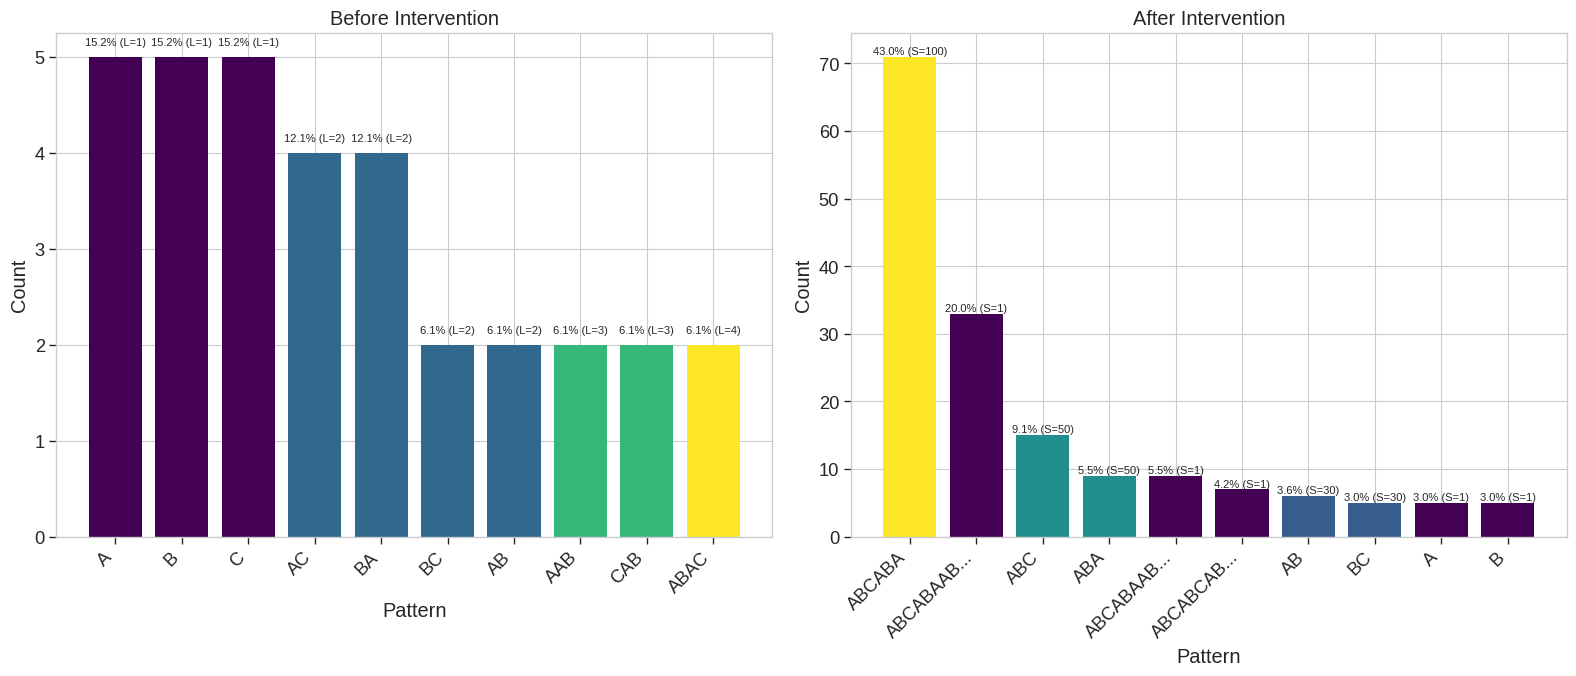
\includegraphics[width=0.9\textwidth]{figure_7.png}
    \caption{Reaction graph for carbon nanostructure assembly, showing progression from carbon monomers to stable nanotube configurations.}
    \label{fig:figure_7}
\end{figure}

Figure~\ref{fig:figure_7} illustrates the progressive assembly of carbon-based structures from simple monomers to complex nanotubes. Carbon atoms (\( \text{C} \)) and hydrogen atoms (\( \text{H} \)) initially form dimers and simple hydrocarbons, which then transform into increasingly complex structures such as benzene (\( \text{C}_6\text{H}_6 \)) and graphene sheets. The pathway culminates in carbon nanotubes, which represent high-stability configurations characterized by exceptional structural integrity.

From an SDA perspective, the stability parameters for compounds increase as the reaction progresses toward more complex structures, reflecting stronger bonding and greater resistance to dissociation. Early products like (\( \text{C}_2 \)) and (\( \text{C}_2\text{H}_4 \)) have relatively short lifetimes, while advanced nanostructures possess significantly higher stability values. This differential stability guides the system toward configurations that persist longer, illustrating how stability-driven selection can shape molecular evolution even without explicit catalytic processes.

\subsection{Pre-RNA Sugar Assembly}

\begin{figure}[h]
    \centering
    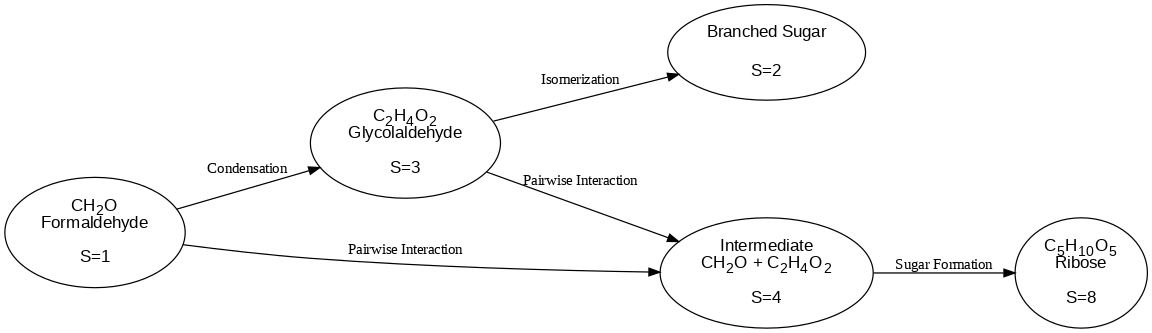
\includegraphics[width=0.9\textwidth]{figure_8.png}
    \caption{Reaction graph for pre-RNA sugar assembly, showing the formation pathway from formaldehyde to ribose.}
    \label{fig:figure_8}
\end{figure}

Figure~\ref{fig:figure_8} presents a simplified reaction network for the formation of ribose, a crucial building block for RNA. The pathway begins with small carbonyl-containing molecules like formaldehyde (CH$_2$O) that condense to form glycolaldehyde (C$_2$H$_4$O$_2$). Through further interactions, these intermediates serve as precursors to ribose (C$_5$H$_{10}$O$_5$). This example is particularly relevant to origins-of-life research, as it illustrates how complex building blocks for genetic polymers might emerge through stability-driven selection.

Both reaction networks demonstrate how SDA systems can model complex chemical pathways by focusing on the stability-determined persistence of intermediates. Rather than tracking every reversible reaction step, the SDA approach highlights how certain "attractor" molecules emerge in branching reaction spaces due to their enhanced stability. This perspective complements traditional kinetic modeling by emphasizing net generational outcomes and selective retention.

It is important to note that in real chemical systems, molecular persistence is influenced by multiple factors beyond intrinsic stability, including energy barriers, temperature, catalytic effects, and external constraints. While SDA systems provide a useful conceptual model, further research is needed to quantify the relative contribution of stability compared to other physical and chemical factors in determining molecular evolution pathways.


\end{document}

\endinput
%%
%% End of file `elsarticle-template-num.tex'.
